\documentclass[11pt,a4paper]{article}

% =========================================================
% PACKAGES
% =========================================================

\usepackage[a4paper,margin=0.8in]{geometry}
\usepackage{graphicx}
\usepackage{float}          % [H] keeps every figure exactly where it is written
\usepackage{booktabs}
\usepackage{array}
\usepackage{enumitem}
\usepackage{amsmath}
\usepackage{amssymb}
\usepackage[hidelinks]{hyperref}
\usepackage{caption}
\usepackage{subcaption}
\usepackage{microtype}

\graphicspath{{figures/}{./}}

\setlength{\parindent}{0pt}
\setlength{\parskip}{5pt}

\setlist[itemize]{
    leftmargin=1.1cm,
    itemsep=1pt,
    topsep=3pt
}

\captionsetup{
    font=small,
    skip=4pt
}

\setcounter{tocdepth}{2}

\begin{document}

% =========================================================
% TITLE PAGE
% =========================================================

\begin{titlepage}

    \centering

    {\Large\textbf{Khulna University of Engineering \& Technology}}\\[0.25cm]

    {\large Department of Computer Science and Engineering}\\[1.4cm]

    % Uncomment if the KUET logo is available
    % \includegraphics[width=0.16\textwidth]{kuet_logo.png}\\[0.8cm]

    {\Large\textbf{Computer Graphics Project Report}}\\[0.7cm]

    {\Huge\textbf{The Trial of Three Curses}}\\[0.45cm]

    {\large An Interactive 3D Adventure Using OpenGL}\\[1.5cm]

    \begin{tabular}{ll}

        \textbf{Course Title:} & Computer Graphics \\

        \textbf{Course Code:} & [Course Code] \\

        \textbf{Submitted To:} & [Teacher Name] \\

        \textbf{Submitted By:} & [Student/Team Name] \\

        \textbf{Roll:} & 2107118 \\

        \textbf{Department:} & Computer Science and Engineering \\

    \end{tabular}

    \vfill

    {\large\textbf{Khulna University of Engineering \& Technology}}\\

    Khulna, Bangladesh\\[0.25cm]

    October 2026

\end{titlepage}


% =========================================================
% ACKNOWLEDGMENT
% =========================================================

\section*{Acknowledgment}
\addcontentsline{toc}{section}{Acknowledgment}

We would like to express our sincere gratitude to our course instructor,
\textbf{[Teacher Name]}, for the guidance, suggestions, and feedback provided
throughout the development of this project. The project gave us the opportunity
to apply both fundamental and advanced computer graphics concepts within a
complete interactive real-time application.

During the development of \textit{The Trial of Three Curses}, we worked with
3D transformations, hierarchical modeling, coordinate systems, camera control,
lighting and shading, shadow mapping, textures, normal mapping, particle
animation, post-processing, procedural effects, collision detection, and
ray-traced reflection. We also acknowledge the use of OpenGL, GLFW, GLAD, and
GLM, which provided the rendering, window-management, input, and mathematical
support required for the implementation.

\clearpage


% =========================================================
% TABLE OF CONTENTS
% =========================================================

\tableofcontents

\clearpage
\setcounter{page}{1}


% =========================================================
% 1. INTRODUCTION
% =========================================================

\section{Introduction}

\subsection{Project Overview}

\textit{The Trial of Three Curses} is an interactive real-time 3D adventure
developed in C++ using OpenGL. The project is inspired by Egyptian and
mythological themes and combines graphics techniques with an environment that
changes continuously as the player progresses. Instead of demonstrating
transformations, lighting, particles, or shaders as isolated examples, these
techniques are integrated into objects, characters, hazards, puzzles, and
cinematic events within the same application.

The adventure begins inside the chamber of Anubis. The traveller places a
glowing heart on a weighing scale, where the result of the judgement determines
whether the traveller is considered balanced or cursed. A successful judgement
awakens a particle-based Djinn from a magical lamp. The Djinn reveals a
treasure and provides a protective charm. When the treasure is collected, the
chamber begins to collapse and the environment becomes dangerous. Large
structural pieces fall from the chamber, smaller debris appears around the
traveller, and Medusa begins pursuing the player while periodically using a
petrifying gaze. The traveller must use pillars and other environmental
features as protection while moving toward the final gate.

At the constellation gate, the Djinn's charm creates a temporary sanctuary
that prevents Medusa from entering. The player must then solve a puzzle
consisting of three rotating rings while fireflies form visual clues around the
gate. Solving the puzzle reveals the Garden of Lost Souls, a second major
environment that is initially dry and lifeless. The traveller offers the
treasure at an Ankh altar, causing a wave of life to spread through the garden.
Plants recover, flowers open, relics begin to glow, the pool becomes reflective,
and seven petrified travellers gradually release their souls. The environment
then transitions from night to dawn.

The garden introduces one of the more advanced rendering techniques of the
project: a shader-based ray-traced reflection system for the pool. Reflection
rays are tested against simplified representations of the surrounding garden
objects, allowing the water to reflect geometry, lighting, sky colour, and
shadows. After sunrise, a reflected sun ray strikes the traveller and begins
the final ascension. The traveller transforms into a soul, rises above the
temple and through the clouds, joins a river of souls leading toward Ra's sun
boat, and eventually becomes the central star of a constellation representing
his journey. The complete project therefore combines graphics mathematics,
real-time rendering, animation, interaction, ray tracing, and visual
storytelling within one continuous experience.

\subsection{Objectives}

The main objectives of the project were:

\begin{itemize}

    \item To construct an interactive real-time 3D environment using OpenGL.

    \item To apply translation, rotation, scaling, composition, and
    hierarchical transformations to scene objects.

    \item To demonstrate model, world, view, and projection coordinate
    transformations.

    \item To implement perspective, free-fly, orbit, first-person, and
    cinematic camera behaviour.

    \item To implement real-time Blinn--Phong lighting using directional,
    point, and spot lights.

    \item To generate dynamic shadows using shadow mapping.

    \item To apply textures, specular maps, and tangent-space normal maps to
    improve surface appearance.

    \item To create particle-based and procedural animations for magical,
    environmental, and cinematic effects.

    \item To implement interactive hazards, collision detection,
    line-of-sight testing, and visual feedback.

    \item To implement shader-based ray-traced reflections for the garden pool.

    \item To integrate the graphics techniques into a complete visual
    narrative rather than isolated demonstrations.

\end{itemize}


% =========================================================
% 2. PROJECT DESIGN AND ARCHITECTURE
% =========================================================

\section{Project Design and Architecture}

The project was designed as a collection of cooperating systems rather than a
single large rendering routine. Game-state management controls the current
stage of the adventure, while separate components are responsible for player
movement, Medusa behaviour, scene construction, camera control, lighting,
shadow generation, particles, environmental destruction, puzzles, garden
animation, and the final ascension. This separation makes it possible for
multiple effects to operate simultaneously without placing unrelated behaviour
inside the same component.

For example, Medusa's physical movement is handled independently from her gaze
attack. Similarly, large predefined structural sections are controlled by the
collapse system, whereas smaller falling stones are handled by the debris
system. The gate puzzle manages ring alignment and clue fireflies separately
from the sanctuary itself. The final garden and ascension systems also reuse
the same scene, material, lighting, particle, and camera infrastructure used
earlier in the chamber.

\subsection{Conceptual Architecture}

Figure~\ref{fig:architecture} presents the high-level architecture of the
project. User input and current game state determine which character and
environmental systems are active. These systems modify the scene objects and
their transformations, after which the camera, lighting, shadow, and shader
systems generate the final rendered image.

\begin{figure}[H]
    \centering
    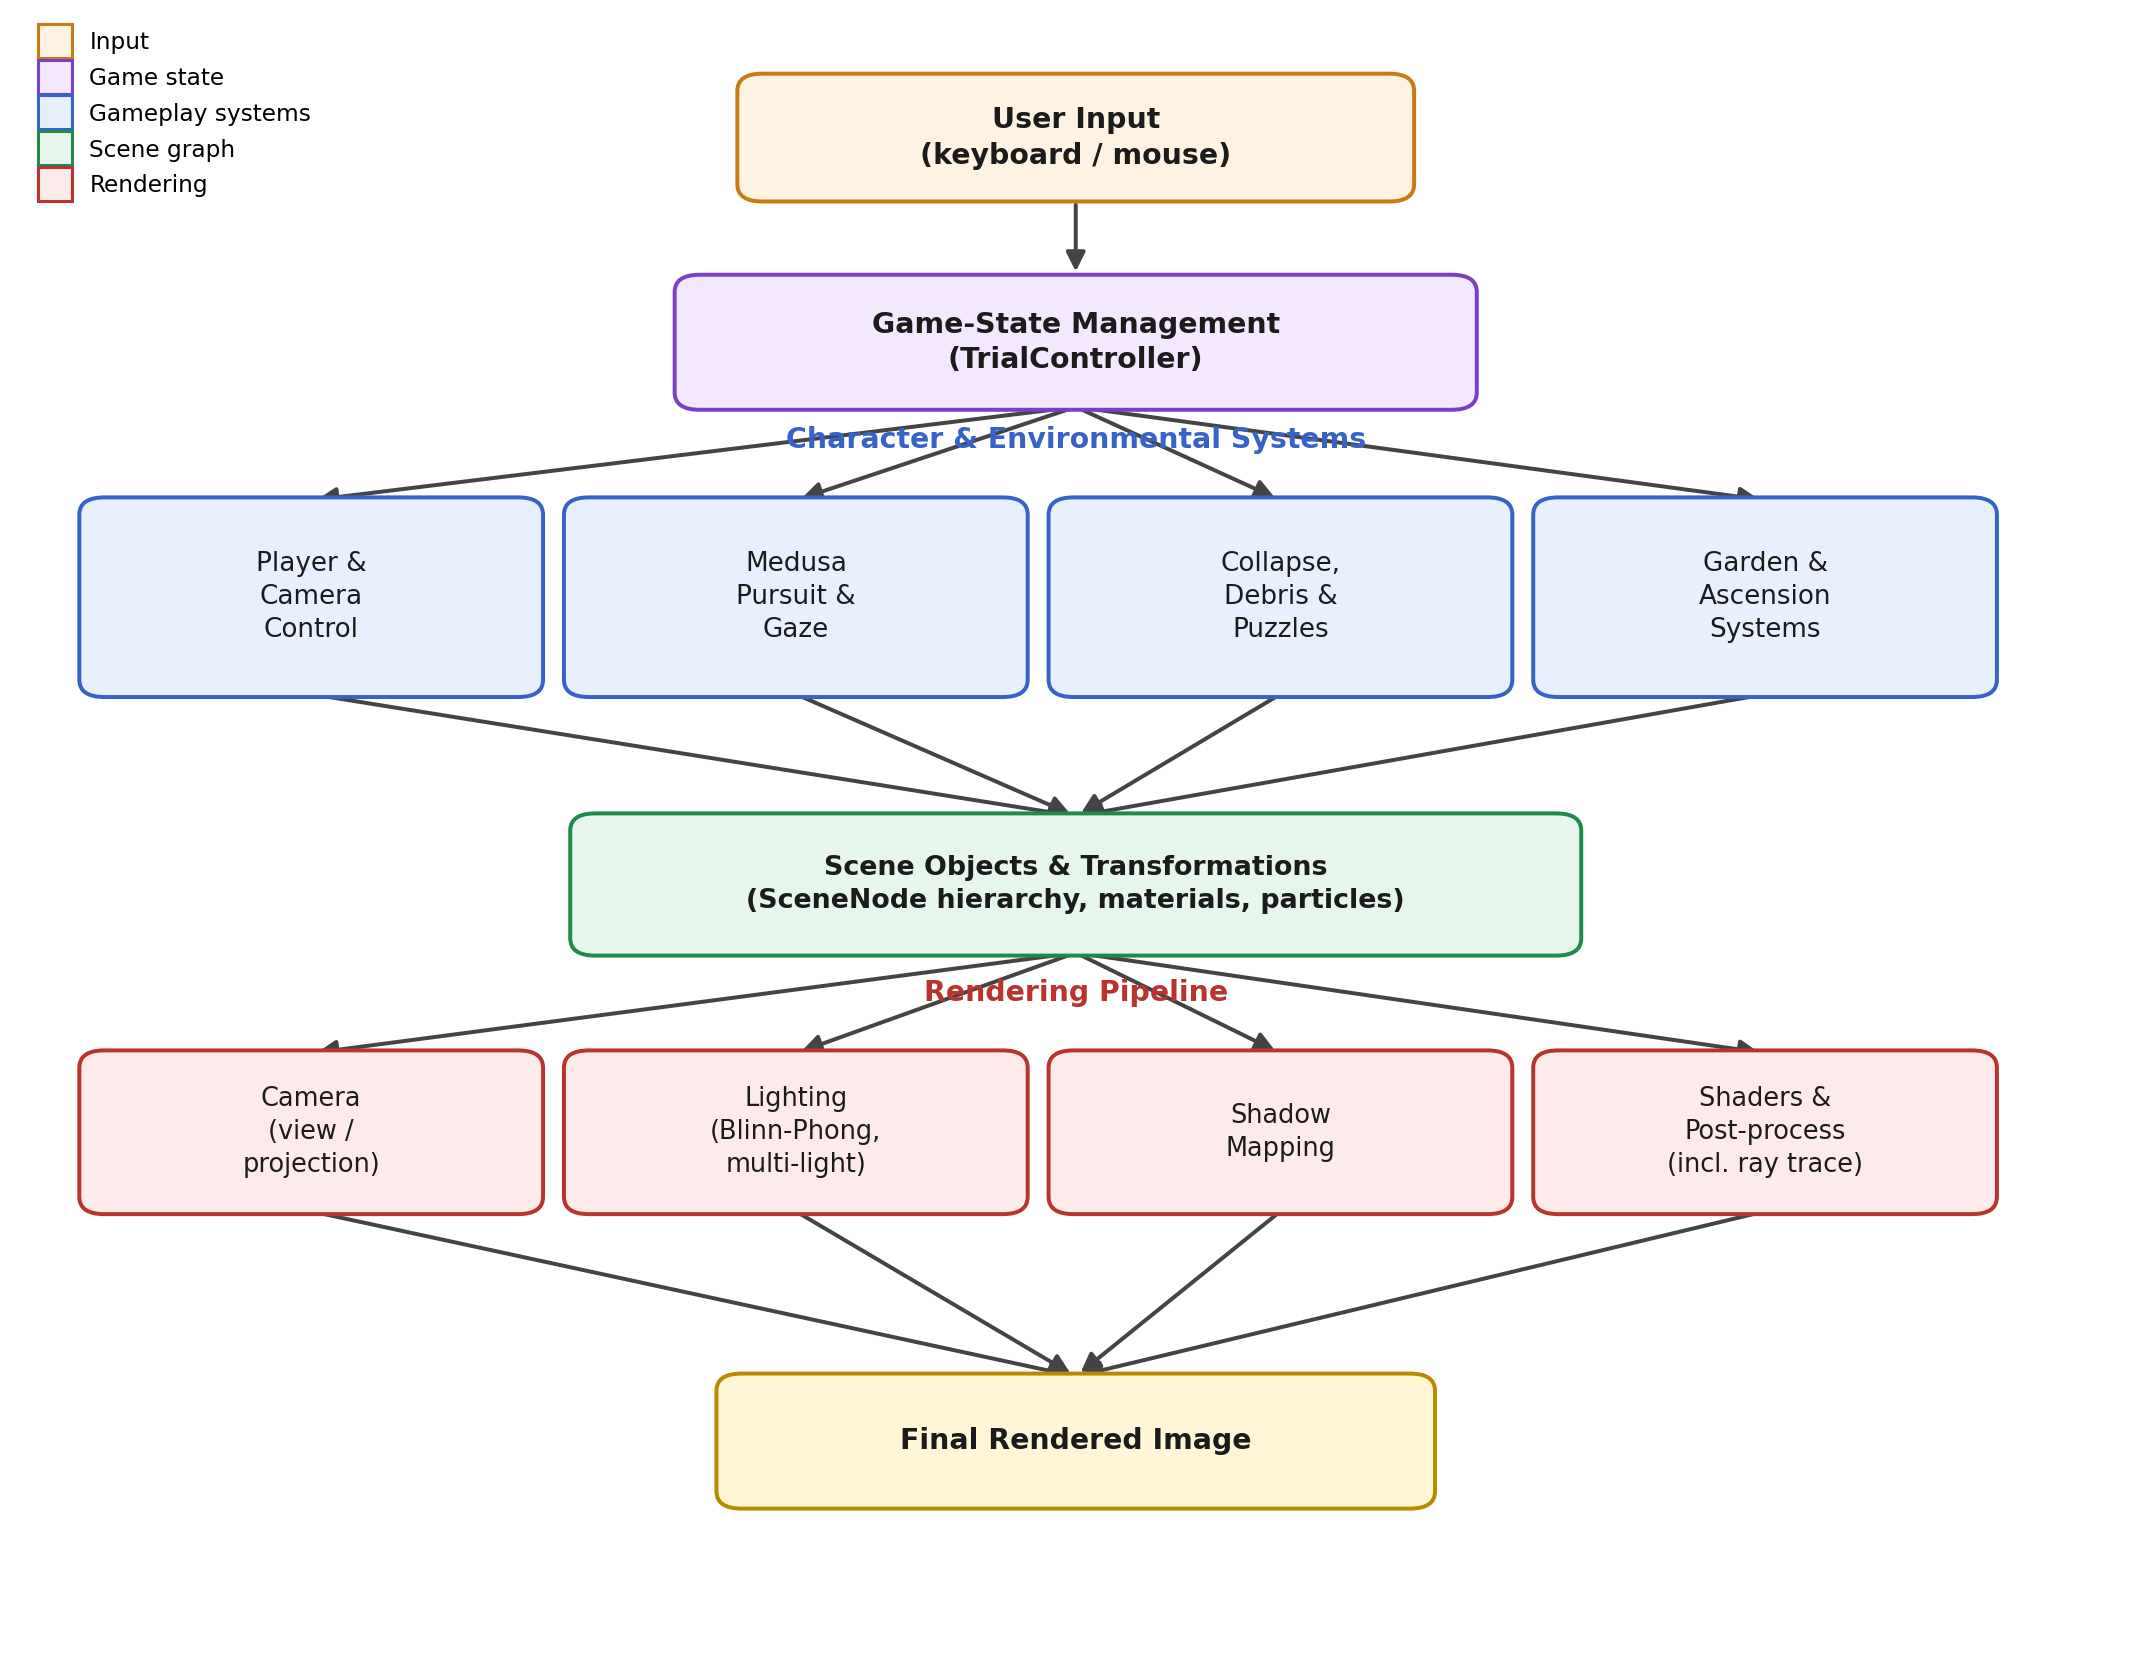
\includegraphics[width=0.93\textwidth]{archi.png}
    \caption{Conceptual architecture of \textit{The Trial of Three Curses}.}
    \label{fig:architecture}
\end{figure}

The application uses an OpenGL 3.3 core-profile rendering context
\cite{opengl}. GLFW \cite{glfw} is used for window creation and input
handling, GLAD \cite{glad} loads the required OpenGL functions, and GLM
\cite{glm} provides vector and matrix operations. The project also contains
specialised vertex, fragment, depth, particle, HUD, and post-processing
shaders. The main rendering path remains rasterization-based, while the garden
pool performs reflection-ray calculations inside its fragment shader.

\subsection{User Interaction and Inspection Controls}

The application provides normal gameplay controls together with inspection
controls used to demonstrate individual graphics features during development
and evaluation. In free-camera mode, movement keys fly the camera instead of
moving the traveller.

\begin{table}[H]
    \centering
    \small
    \begin{tabular}{p{0.25\textwidth} p{0.62\textwidth}}
        \toprule
        \textbf{Control} & \textbf{Function} \\
        \midrule
        WASD / Arrow keys & Move the traveller relative to the camera; in free-camera mode, fly the camera \\
        Left mouse drag / Scroll & Rotate the view and control zoom \\
        TAB & Cycle cinematic, first-person, and free-camera views \\
        SPACE & Begin the scale trial or show the gate clue when applicable \\
        Arrow keys at gate & Select and rotate the puzzle rings; WASD still moves the traveller \\
        R & Reset the current trial \\
        G & Toggle shadow mapping \\
        V & Toggle normal mapping \\
        U & Toggle post-processing \\
        Z & Toggle ray-traced pool reflection \\
        Y & Toggle textures \\
        N & Display surface normals for inspection \\
        \bottomrule
    \end{tabular}
    \caption{Main gameplay and graphics-inspection controls.}
    \label{tab:controls}
\end{table}


% =========================================================
% 3. GRAPHICS DESIGN AND IMPLEMENTATION
% =========================================================

\section{Graphics Design and Implementation}

% ---------------------------------------------------------
% 3.1 Scene Modeling and Transformations
%     Figure: wireframe / untextured / final
% ---------------------------------------------------------

\subsection{Scene Modeling and Transformations}

The project environment is constructed from reusable geometric primitives such
as cubes, spheres, cylinders, cones, toruses, and planes. These primitives are
combined to form more complex objects including the Anubis scale, lamp,
traveller, Medusa, gate, garden vegetation, relics, Ra's sun boat, and Ba
birds. This approach allows the project to create a large number of different
visual objects without depending entirely on external 3D models.

Each scene object stores a position, rotation, and scale. The local model
transformation can be written as

\begin{equation}
    M = TRS ,
\end{equation}

where $T$, $R$, and $S$ are the translation, rotation, and scaling matrices,
respectively. Translation is used for objects such as the traveller, Medusa,
debris, released souls, and the ascension orb. Rotation is used extensively for
the scale beam, lamp lid, gate rings, falling structures, sun-boat oars, and
Ba-bird wings. Scaling is used for effects including the heart pulse, particle
formation, plant restoration, disappearance of the traveller's body, and
several magical effects.

Figure~\ref{fig:model_render_comparison} shows the same environment at
different stages of rendering. The wireframe view exposes the polygonal
structure of the scene, while disabling textures shows the contribution of
material and lighting alone. The final view combines the geometry with the
texture and shading information used during normal rendering.

\begin{figure}[H]
    \centering
    \begin{subfigure}[t]{0.32\textwidth}
        \centering
        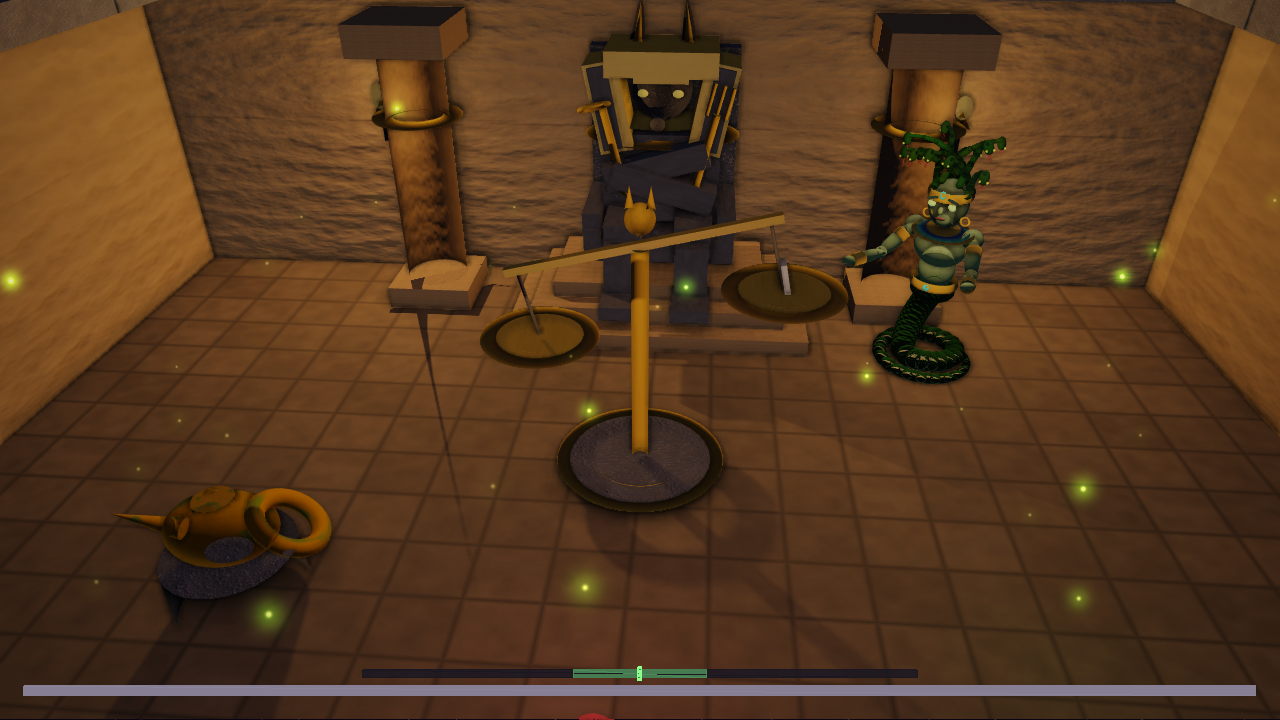
\includegraphics[width=\linewidth]{wireframe_view.png}
        \caption{Wireframe geometry.}
    \end{subfigure}
    \hfill
    \begin{subfigure}[t]{0.32\textwidth}
        \centering
        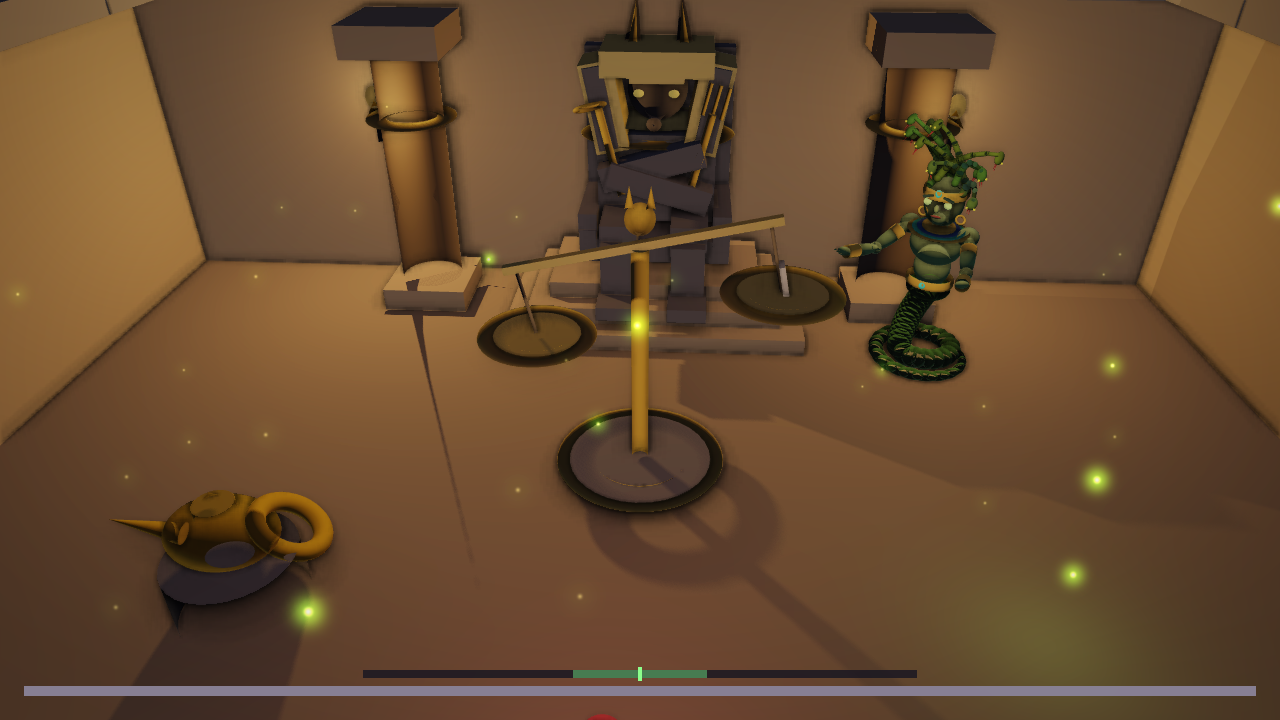
\includegraphics[width=\linewidth]{without_texture.png}
        \caption{Textures disabled.}
    \end{subfigure}
    \hfill
    \begin{subfigure}[t]{0.32\textwidth}
        \centering
        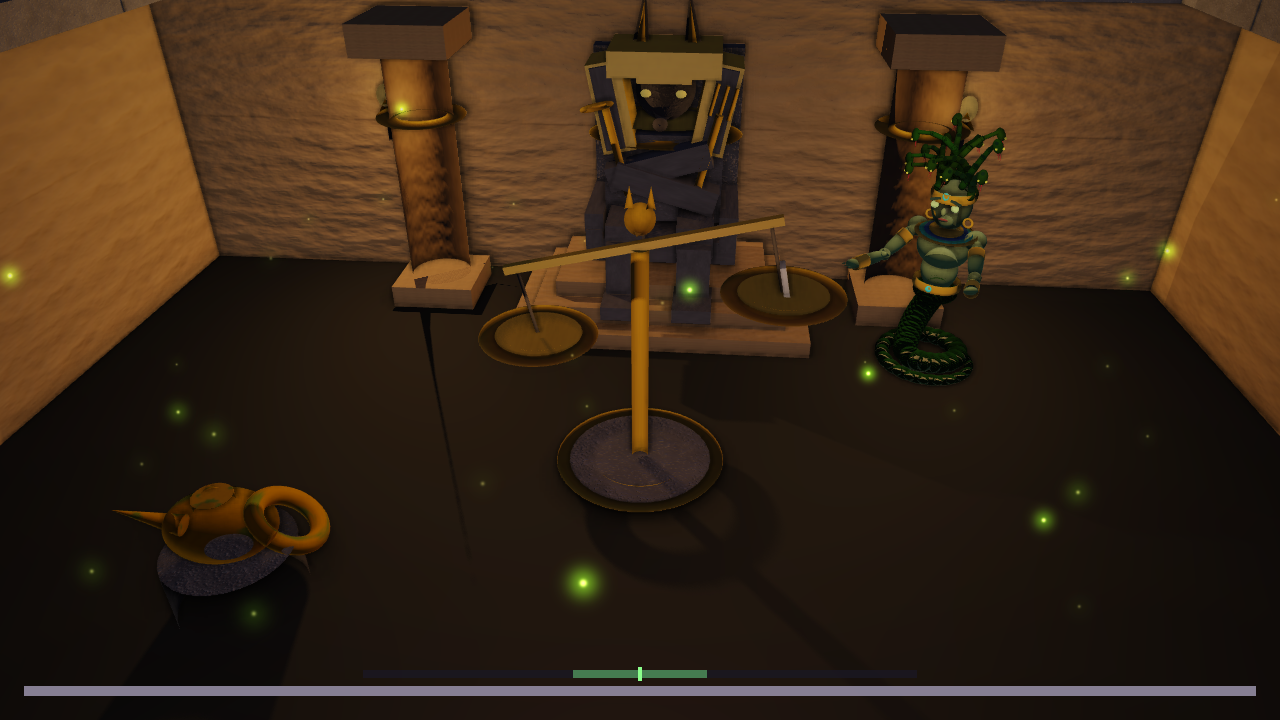
\includegraphics[width=\linewidth]{with_texture.png}
        \caption{Final textured rendering.}
    \end{subfigure}
    \caption{Visual effect of the main scene representation:
    (a) underlying polygonal geometry,
    (b) solid shaded geometry without texture mapping, and
    (c) the final textured scene.}
    \label{fig:model_render_comparison}
\end{figure}

Back-face culling is enabled during normal rendering so that triangles facing
away from the viewer are not unnecessarily processed. Counter-clockwise
triangles are treated as front-facing, while back-facing triangles are
discarded. Certain double-sided objects temporarily disable culling when both
sides must remain visible.

% Optional: enable this block if you have back-face culling screenshots.
% File names are placeholders -- rename them to match your images.
%
% Figure~\ref{fig:culling_comparison} compares the same view with back-face
% culling disabled and enabled.
%
% \begin{figure}[H]
%     \centering
%     \begin{subfigure}[t]{0.48\textwidth}
%         \centering
%         \includegraphics[width=\linewidth]{culling_off.png}
%         \caption{Back-face culling disabled.}
%     \end{subfigure}
%     \hfill
%     \begin{subfigure}[t]{0.48\textwidth}
%         \centering
%         \includegraphics[width=\linewidth]{culling_on.png}
%         \caption{Back-face culling enabled.}
%     \end{subfigure}
%     \caption{Effect of back-face culling on the rendered scene.}
%     \label{fig:culling_comparison}
% \end{figure}

% ---------------------------------------------------------
% 3.2 Hierarchical Modeling  (no figure)
% ---------------------------------------------------------

\subsection{Hierarchical Modeling}

Complex objects are represented through parent--child relationships using the
scene graph. A child first applies its local transformation and then inherits
the transformation of its parent. Therefore, its final world transformation is

\begin{equation}
    M_{\mathrm{world}}
    =
    M_{\mathrm{parent}}M_{\mathrm{local}} .
\end{equation}

Anubis's scale is one of the clearest examples. The pans are connected to the
scale structure, while the heart and feather move relative to their respective
pans. When the scale beam rotates, its children follow automatically. The pans
apply an opposite rotation so that they remain approximately horizontal while
the beam tilts. The same hierarchical principle appears throughout the project.
The lamp lid rotates about its hinge, collapsing structures rotate around
attachment points before detaching, the boat's oars are connected to pivot
nodes, and each Ba bird has wing pivots attached to its body. As a result, a
single parent rotation can animate an entire connected structure.

% ---------------------------------------------------------
% 3.3 Coordinate Systems and Camera  (no figure)
% ---------------------------------------------------------

\subsection{Coordinate Systems and Camera}

The renderer uses the standard sequence of model, world, view, and projection
transformations. A vertex is initially defined relative to its own object. The
model matrix places it into world space, the view matrix expresses the world
relative to the camera, and the projection matrix converts the result into the
perspective view required for rasterization. The complete transformation is

\begin{equation}
    P_{\mathrm{clip}}
    =
    P_{\mathrm{projection}}
    V_{\mathrm{view}}
    M_{\mathrm{model}}
    P_{\mathrm{local}} .
\end{equation}

The camera view matrix is generated from the camera position, target, and
world-up vector using \texttt{glm::lookAt()}, while perspective projection is
created using \texttt{glm::perspective()} \cite{glm}. Yaw controls horizontal
viewing direction and pitch controls vertical direction. The project supports
cinematic, first-person, and free-camera views, while the underlying camera
also supports orbit and free-fly behaviour.

Cinematic camera control is particularly important because the environment
changes substantially throughout the project. During the Anubis trial, the
camera emphasises the scale and heart; during the escape it follows the moving
traveller and threats; in the garden it frames the altar, restoration wave, and
souls; and during ascension it moves above the temple, through the cloud layer,
toward the sun boat, and finally into the constellation scene. Smooth changes
in camera target, distance, yaw, and pitch avoid sudden transitions and make
the events easier to follow.

% ---------------------------------------------------------
% 3.4 Materials, Textures and Normal Mapping
%     Figure: normal mapping OFF / ON
% ---------------------------------------------------------

\subsection{Materials, Textures and Normal Mapping}

Scene objects use materials containing ambient, diffuse, specular, emissive,
and shininess properties. Gold is assigned stronger specular reflection and a
higher shininess value than rough stone, allowing objects constructed from the
same basic geometry to respond differently to the same light source. Emissive
values are used for objects that need to appear self-lit, such as magical
energy, Medusa's eyes, fireflies, stars, debris warnings, and parts of the sun
boat.

The project also uses procedurally generated diffuse, specular, and normal
textures. Sandstone, floor tiles, gold, brass, stone, and snake surfaces receive
different texture information. Normal maps perturb the surface normal inside
the fragment shader using a tangent--bitangent--normal basis. This creates the
appearance of small-scale surface relief without increasing the number of
geometric polygons. The normal maps can also be disabled during execution,
making it possible to compare the shaded surface with and without the added
detail.

Figure~\ref{fig:normalmap_comparison} compares the same view with normal
mapping disabled and enabled. The geometry is identical in both images; only
the normals used by the lighting calculation are perturbed, which produces the
additional surface relief.

\begin{figure}[H]
    \centering
    \begin{subfigure}[t]{0.48\textwidth}
        \centering
        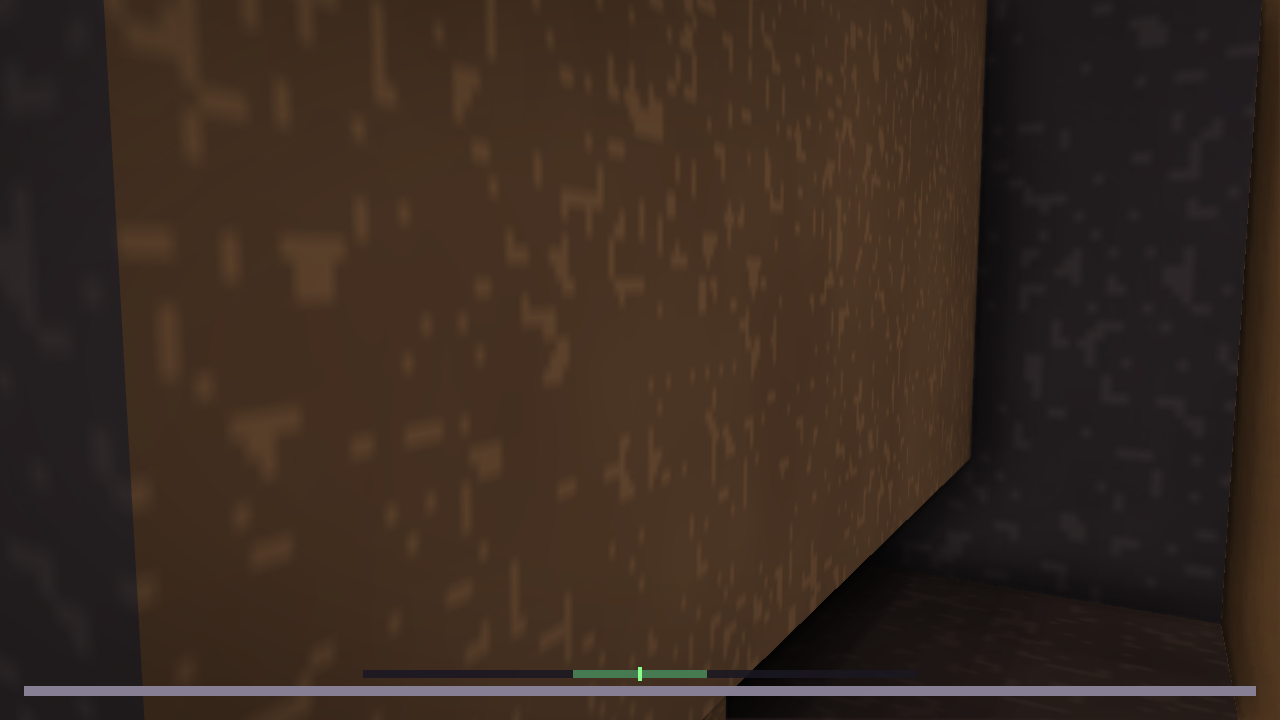
\includegraphics[width=\linewidth]{normalmap_off.png}
        \caption{Normal mapping disabled.}
    \end{subfigure}
    \hfill
    \begin{subfigure}[t]{0.48\textwidth}
        \centering
        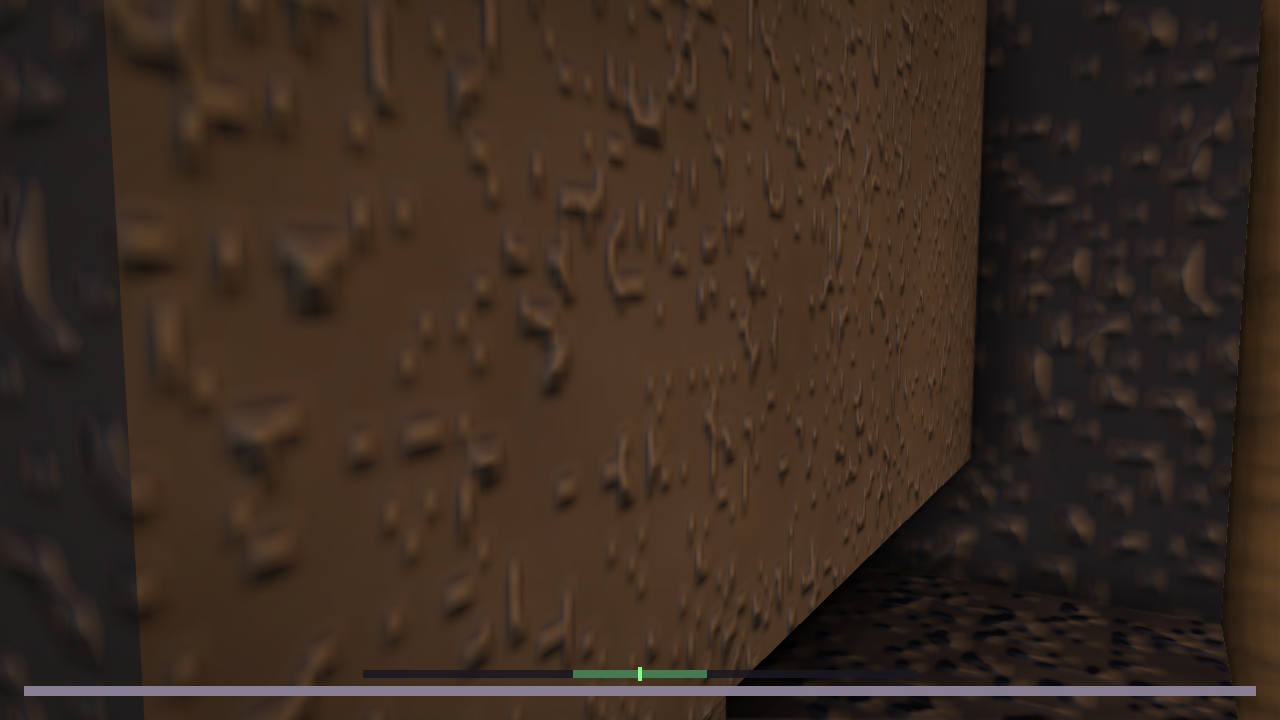
\includegraphics[width=\linewidth]{normalmap_on.png}
        \caption{Normal mapping enabled.}
    \end{subfigure}
    \caption{Effect of tangent-space normal mapping on surface shading.}
    \label{fig:normalmap_comparison}
\end{figure}

For correct lighting under non-uniform scaling, surface normals are transformed
using the inverse-transpose of the model matrix,

\begin{equation}
    N_{\mathrm{world}}
    =
    \left(M^{-1}\right)^{T}N_{\mathrm{local}} .
\end{equation}

This prevents scaling operations, such as the pulsing heart and growing objects,
from incorrectly distorting the surface normals.

% ---------------------------------------------------------
% 3.5 Lighting and Blinn--Phong Shading
%     Equations and explanation only (no artificial comparison)
% ---------------------------------------------------------

\subsection{Lighting and Blinn--Phong Shading}

The scene uses directional, point, and spot lights. Directional lighting is
used for broad environmental illumination, including the transition toward
morning in the garden. Point lights are used for local sources such as torches,
the glowing heart, treasure, charm, selected fireflies, and other magical
effects. Spot lighting is used for directional effects including Medusa's
eye-related illumination.

For point and spot lights, intensity decreases with distance using

\begin{equation}
    A(d)
    =
    \frac{1}{k_c+k_l d+k_qd^2},
\end{equation}

where $d$ is the distance to the light, while $k_c$, $k_l$, and $k_q$ are the
constant, linear, and quadratic attenuation terms.

The main surface shader uses a Blinn--Phong lighting model \cite{learnopengl}.
The total illumination can be described as

\begin{equation}
    I = I_a + I_d + I_s ,
\end{equation}

where $I_a$, $I_d$, and $I_s$ are the ambient, diffuse, and specular
components. Diffuse illumination depends on the angle between the surface
normal $\vec{N}$ and the light direction $\vec{L}$,

\begin{equation}
    I_d \propto \max(\vec{N}\cdot\vec{L},0),
\end{equation}

The Blinn--Phong half-vector is calculated from the normalized light and view
directions as

\begin{equation}
    \vec{H}
    =
    \frac{\vec{L}+\vec{V}}
    {\|\vec{L}+\vec{V}\|}.
\end{equation}

The specular term then uses this half-vector,

\begin{equation}
    I_s \propto
    \max(\vec{N}\cdot\vec{H},0)^{s},
\end{equation}

where $s$ is the material shininess. Spotlights also use inner and outer cone
limits to create a soft edge rather than an abrupt boundary. Together, these
techniques allow the same lighting system to support dark stone chambers,
magical cyan effects, warm golden surfaces, the restored garden, and the final
sky environment.

% ---------------------------------------------------------
% 3.6 Shadow Mapping
%     Figure: shadow OFF / ON
% ---------------------------------------------------------

\subsection{Shadow Mapping}

Real-time shadows are generated using shadow mapping. The scene is first
rendered from the position of the shadow-casting light, where the depth of the
closest visible surface is stored in a depth texture. During the normal camera
render, each fragment is transformed into the same light-space coordinate
system and its depth is compared with the corresponding value stored in the
shadow map. If the current fragment is farther from the light than the stored
surface, another object lies between the fragment and the light, and the
fragment is therefore treated as shadowed and receives reduced direct
illumination.

The implementation uses a slope-dependent depth bias to reduce self-shadowing
artifacts. Surfaces that face away from the light require a larger bias than
surfaces facing it directly. The shader also performs a $3\times3$
percentage-closer filtering operation, averaging nine nearby depth tests to
soften the otherwise hard and stair-stepped shadow boundary. Shadow mapping is
especially useful inside the chamber, where pillars, characters, walls, and
large props create strong depth cues under the scene lighting.

The effect can be observed directly by rendering the same scene with shadow
mapping disabled and enabled, as shown in
Figure~\ref{fig:shadow_comparison}. The geometry, materials, camera, and light
positions remain unchanged, so the visible difference is produced by the
shadow test.

\begin{figure}[H]
    \centering
    \begin{subfigure}[t]{0.48\textwidth}
        \centering
        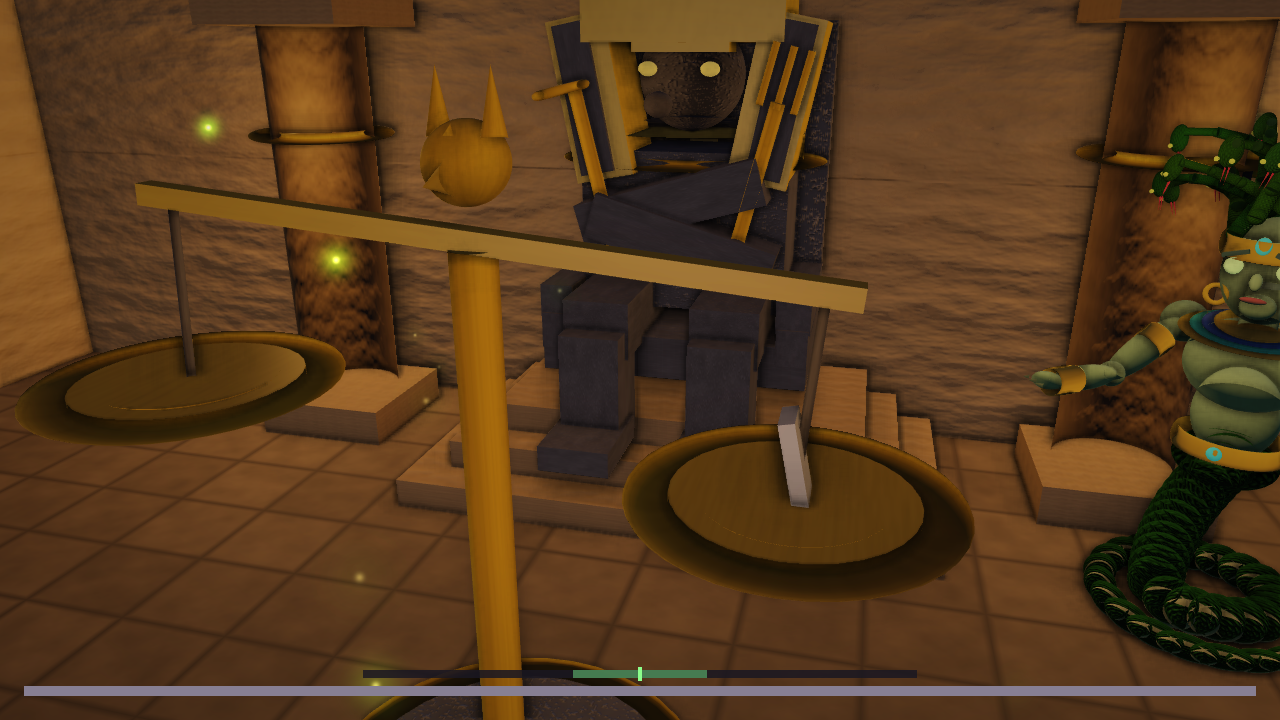
\includegraphics[width=\linewidth]{without_shadow.png}
        \caption{Shadow mapping disabled.}
    \end{subfigure}
    \hfill
    \begin{subfigure}[t]{0.48\textwidth}
        \centering
        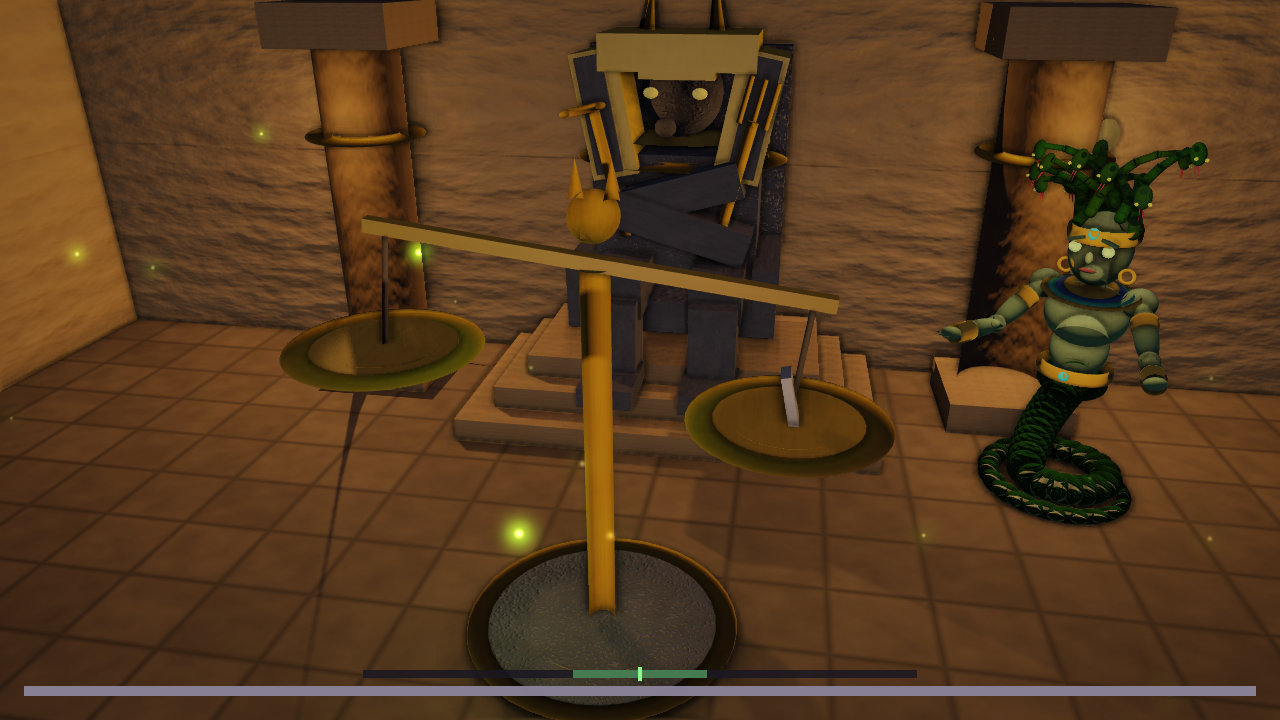
\includegraphics[width=\linewidth]{with_shadow.png}
        \caption{Shadow mapping enabled.}
    \end{subfigure}

    \caption{Comparison of the same chamber view without and with shadow
    mapping. Shadows provide clearer spatial relationships between objects
    and improve depth perception.}
    \label{fig:shadow_comparison}
\end{figure}

% ---------------------------------------------------------
% 3.7 Particle and Procedural Animation  (no figure here;
%     particle results appear in Section 5)
% ---------------------------------------------------------

\subsection{Particle and Procedural Animation}

Particles are used when a rigid mesh would not provide the required visual
behaviour. The Djinn is the largest early example: instead of appearing as one
solid model, it is assembled from particles representing different body
regions, including the tail, torso, head, arms, hands, beard, turban, and eyes.
Each particle has a desired target location and moves toward that location using
spring-like acceleration,

\begin{equation}
    \vec{a}
    =
    k(\vec{x}_{t}-\vec{x})-c\vec{v},
\end{equation}

where $\vec{x}_{t}$ is the target position, $\vec{x}$ is the current position,
$\vec{v}$ is the velocity, $k$ controls the attraction strength, and $c$
provides damping. Sine and cosine functions introduce small changes in position
so that the final form continues to swirl and breathe instead of becoming
perfectly static.

The same particle infrastructure is reused for other effects, but with
different behaviour. Fireflies wander and blink, gate fireflies move into clue
patterns, impacts generate dust and fragments, petrified statues release golden
particles, souls rise while leaving trails, the reflected sun ray is drawn from
many small glows, and the final ascension contains a river of 150 glowing
souls. Reusing the particle renderer in this way allowed visually different
effects to be created without developing a completely separate renderer for
each event.

For rendering, particles are represented as small camera-facing billboard
quads rather than individual 3D meshes. The camera's right and up vectors are
used to orient each quad toward the viewer, while particle position, size, and
colour are supplied as per-instance data. The particles are drawn using
instanced rendering, allowing many particles to be rendered with a small
number of draw calls. Additive blending is used for glowing effects so that
overlapping particles increase the visible brightness of Djinn energy,
fireflies, souls, and other magical effects.

% ---------------------------------------------------------
% 3.8 Petrification and Post-Processing
%     Figure: post-processing OFF / ON
% ---------------------------------------------------------

\subsection{Petrification and Post-Processing}

Medusa's curse includes both an object-level and a full-screen graphics effect.
For the traveller, petrification is calculated per fragment using the world
height of the current pixel. As the petrification value increases, a conversion
front moves upward from the traveller's feet. Material properties are blended
from flesh to stone around this front, allowing part of the same limb to remain
flesh while the lower part has already become stone. A coloured emissive edge
is added around the moving boundary so that the progression is clearly visible.

The composed scene is then passed through a post-processing shader. As the
curse becomes stronger, the entire frame gradually loses colour, a vignette
darkens the corners, and the image receives a stone-like tint. This full-screen
effect is important because the curse visually affects the player's complete
view rather than only the traveller model. The same system is adjusted in the
opposite direction after a successful escape, reducing the vignette and adding
a warmer visual tone.

The full-screen effects are applied using an off-screen framebuffer. The 3D
scene is first rendered into a colour texture with a depth attachment instead
of directly to the screen. After the scene render is complete, this texture is
processed by the post-processing shader using a single full-screen triangle.
This second pass applies the desaturation, vignette, and colour tint uniformly
to the completed frame.

Figure~\ref{fig:post_comparison} compares the same petrification view with
full-screen post-processing disabled and enabled.

\begin{figure}[H]
    \centering
    \begin{subfigure}[t]{0.48\textwidth}
        \centering
        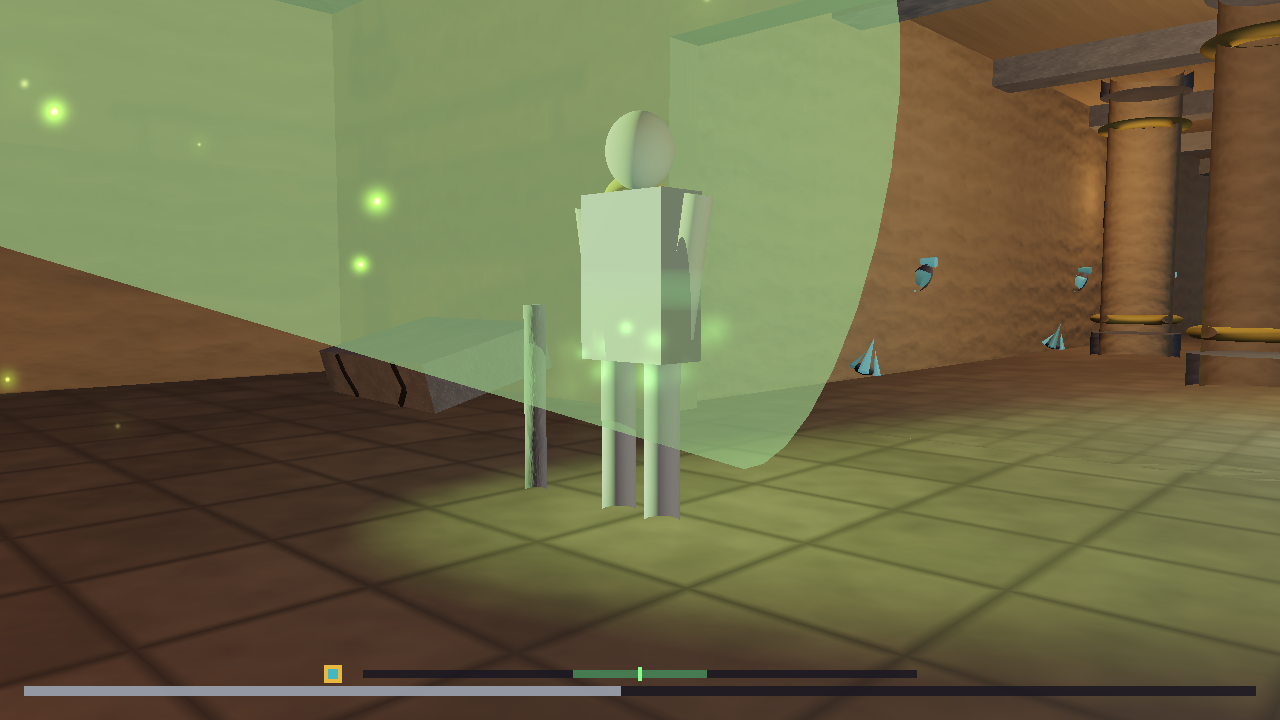
\includegraphics[width=\linewidth]{post_off.png}
        \caption{Post-processing disabled.}
    \end{subfigure}
    \hfill
    \begin{subfigure}[t]{0.48\textwidth}
        \centering
        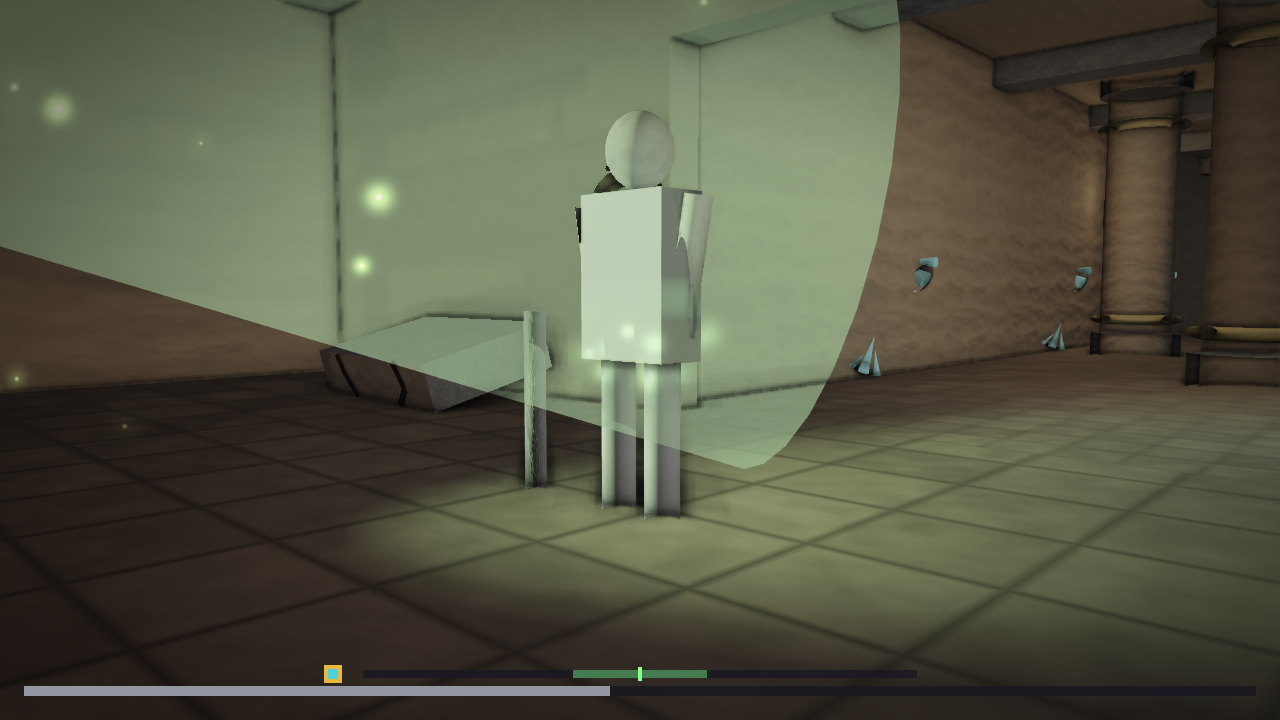
\includegraphics[width=\linewidth]{post_on.png}
        \caption{Post-processing enabled.}
    \end{subfigure}
    \caption{Effect of the full-screen petrification post-process.}
    \label{fig:post_comparison}
\end{figure}

% ---------------------------------------------------------
% 3.9 Ray-Traced Pool Reflection
%     Figure: ray tracing OFF / ON
% ---------------------------------------------------------

\subsection{Ray-Traced Pool Reflection}

The Garden of Lost Souls contains a water surface that uses actual reflection
rays inside the fragment shader. For each relevant water fragment, a ray is
described as

\begin{equation}
    P(t)=O+tD ,
\end{equation}

where $O$ is the ray origin and $D$ is its direction. The reflected ray
direction is calculated using the law of reflection,

\begin{equation}
    \vec{R}
    =
    \vec{I}
    -
    2(\vec{N}\cdot\vec{I})\vec{N},
\end{equation}

where $\vec{I}$ is the incident viewing direction and $\vec{N}$ is the
perturbed water normal.

Rather than testing the ray against every triangle in the scene, visible garden
objects are converted into simplified ray-tracing geometry. Most objects are
represented as axis-aligned boxes, while sphere-based objects are represented
as ellipsoids. The shader supports up to 48 boxes and 40 ellipsoids. Box
intersection is calculated using the slab method, while ellipsoid intersection
is reduced to a quadratic unit-sphere test. The nearest valid hit determines
the reflected surface colour.

For ellipsoid intersection, the ray is first transformed so that the ellipsoid
becomes a unit sphere,

\begin{equation}
    \vec{o}'=\frac{\vec{O}-\vec{C}}{\vec{r}},
    \qquad
    \vec{d}'=\frac{\vec{D}}{\vec{r}} .
\end{equation}

The intersection is then obtained from

\begin{equation}
    at^2+2bt+c=0,
\end{equation}

where
$a=\vec{d}'\cdot\vec{d}'$,
$b=\vec{o}'\cdot\vec{d}'$, and
$c=\vec{o}'\cdot\vec{o}'-1$.
A valid positive value of $t$ represents a surface hit.

The reflection is not simply an unlit object lookup. After a ray hits a
surface, another ray is sent toward the garden light to determine whether that
reflected point is shadowed. If the reflection ray hits nothing, the sky colour
is used instead. Animated sine and cosine terms slightly modify the water
normal to create ripples, and Fresnel-style mixing makes the reflection
stronger at shallow viewing angles. The complete ray-tracing effect can be
enabled or disabled at runtime, allowing direct comparison with ordinary water
shading.

Figure~\ref{fig:raytracing_comparison} shows the contribution of the
reflection-ray calculation to the garden pool.

\begin{figure}[H]
    \centering
    \begin{subfigure}[t]{0.48\textwidth}
        \centering
        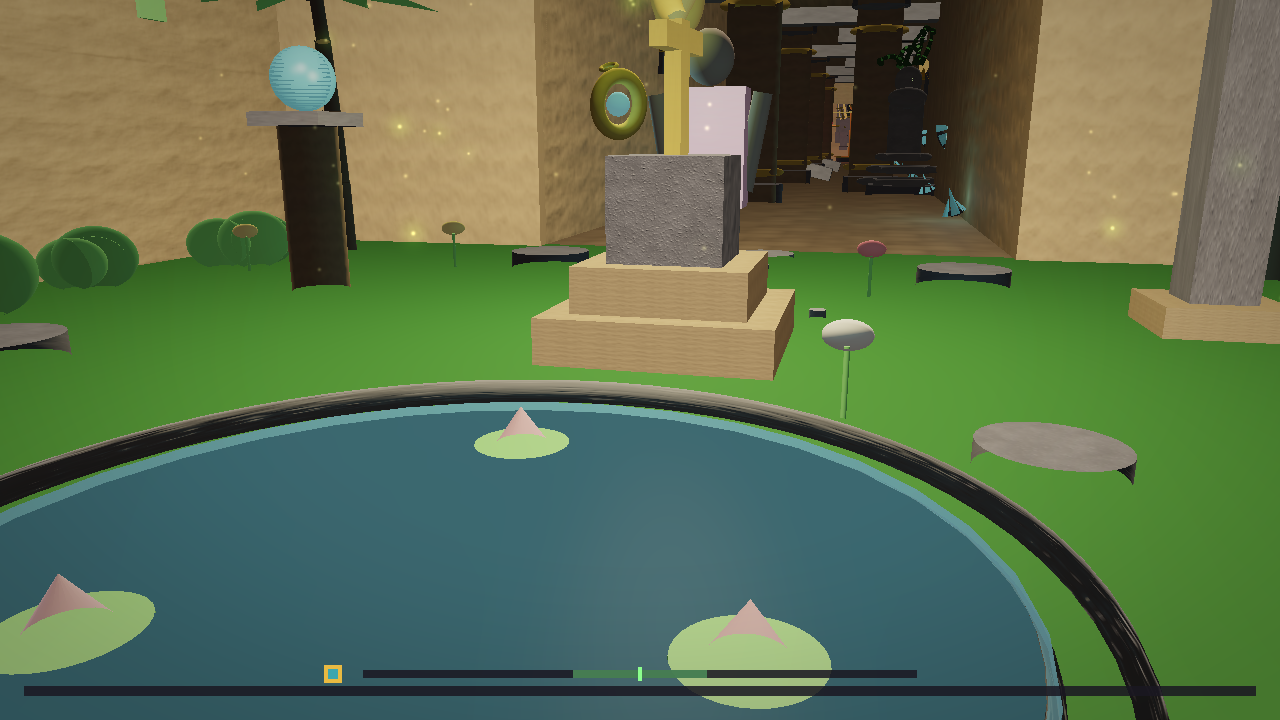
\includegraphics[width=\linewidth]{raytracing_off.png}
        \caption{Pool ray tracing disabled.}
    \end{subfigure}
    \hfill
    \begin{subfigure}[t]{0.48\textwidth}
        \centering
        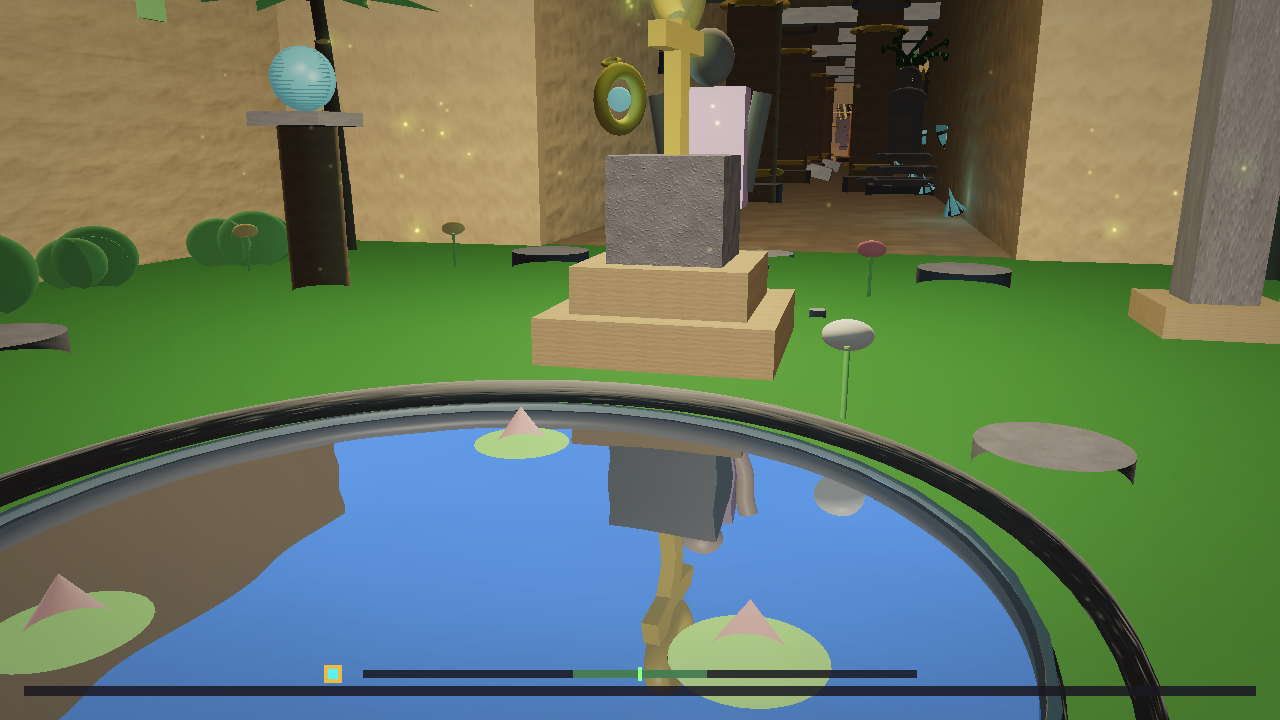
\includegraphics[width=\linewidth]{raytracing_on.png}
        \caption{Pool ray tracing enabled.}
    \end{subfigure}

    \caption{Comparison of the garden pool with and without shader-based
    ray-traced reflection.}
    \label{fig:raytracing_comparison}
\end{figure}


% =========================================================
% 4. INTERACTIVE SYSTEMS AND ENVIRONMENTAL DESIGN
% =========================================================

\section{Interactive Systems and Environmental Design}

\subsection{Anubis Trial, Djinn and Protective Charm}

The Anubis trial is built around the relationship between the traveller, heart,
scale, and environment. When the trial begins, the heart moves from the
traveller toward the scale using smooth interpolation while the scale beam and
pans respond through hierarchical transformations. The glowing heart also acts
as a moving point light, which means that its illumination follows the heart
rather than remaining fixed in the chamber. The result of the judgement affects
the later state of the application: a cursed outcome leads toward
petrification, whereas a balanced result allows the traveller to continue.

Following a successful judgement, the magical lamp opens around its hinge and
the Djinn gradually forms from particles above it. The Djinn then reveals the
treasure and provides the traveller with a small protective charm. The charm is
constructed from a gold band and an emissive cyan gem and remains associated
with the traveller during the escape. It also produces local illumination,
becoming stronger when it later powers the sanctuary around the constellation
gate. This connects an object introduced during the Djinn scene with a
mechanical and visual purpose much later in the adventure.

\subsection{Chamber Collapse and Falling Debris}

Collecting the treasure starts a large environmental destruction sequence.
Major architectural sections are predefined as collapse pieces so that each
one can crack, shake, detach, rotate, fall, and settle while preserving the
overall structure of the chamber. Shaking is produced using oscillating
functions, while the detachment stage rotates a piece around an attached edge
before it becomes independent. Once detached, its vertical movement follows
the usual gravitational relation

\begin{equation}
    y(t)
    =
    y_0-v_0t-\frac{1}{2}gt^2 .
\end{equation}

Smaller falling stones are handled by a separate debris system. These stones
are spawned dynamically, receive downward velocity and rotational motion, and
can become obstacles after reaching the floor. Before impact, a red or orange
emissive warning is drawn at the same horizontal $(x,z)$ position as the
falling stone. The marker becomes more urgent as impact approaches, allowing
the player to understand a three-dimensional danger by looking at a clear
two-dimensional location on the floor. This system makes the collapse
interactive instead of purely decorative.

\subsection{Medusa Pursuit, Gaze and Visibility}

Medusa combines a physical pursuit system with a separate visual threat. During
the chase, her direction is continuously adjusted toward the traveller while
her movement is constrained by the same environment used for player collision.
Local avoidance is applied around fallen rubble and other obstacles so that the
character does not simply move through solid objects. Her heading is smoothed
as the movement direction changes, which prevents unrealistic instantaneous
rotation.

The gaze attack is handled independently from physical pursuit. Medusa's eyes
first signal an incoming attack before the dangerous gaze becomes active. The
system checks whether the traveller lies inside the allowed gaze direction and
then tests visibility through the environment. Pillars are approximated by
vertical blocking volumes, and lines are tested from Medusa toward several
points on the traveller's upper body. Testing multiple points means that a
pillar can provide partial cover instead of producing only a completely visible
or completely hidden result. When enough of the body remains exposed,
petrification grows; when the player reaches cover, the accumulated exposure
gradually decreases. This combines geometric visibility testing with the
fragment-level petrification and full-screen post-processing effects described
earlier.

\subsection{Sanctuary and Constellation Gate}

A traveller who successfully received the Djinn's charm can activate the
sanctuary near the end of the corridor. The charm raises a glowing cyan
protective dome around the gate and keeps Medusa outside while the player solves
the puzzle. The sanctuary is temporary and begins to flicker as its remaining
time becomes low, giving the player visual feedback without requiring a large
text message.

The gate contains three independently rotating rings. Each ring has six valid
orientations, so one discrete step corresponds to

\begin{equation}
    \frac{360^\circ}{6}=60^\circ .
\end{equation}

Gold markers on the rings make their orientations visible. The required
solution is communicated through fireflies rather than through a conventional
text instruction. When the clue is requested, the fireflies move into a small
constellation pattern containing one important location for each ring. Circular
positions around the gate are obtained using sine and cosine, and the rings
interpolate smoothly toward their selected angles. When all three orientations
match the clue and remain aligned, the gate opens by sinking into the floor and
the traveller gains access to the hidden garden.

\subsection{Garden of Lost Souls and Wave of Life}

The Garden of Lost Souls is designed as a visual contrast to the enclosed
chamber. It contains an open night sky, low walls, desert dunes beyond the back
boundary, stepping stones, palm trees, bushes, flowers, lotus plants, wall ivy,
a crystal relic, an obelisk, an Ankh altar, and a pool. Seven stone statues are
placed around the area to represent earlier travellers caught by Medusa. Their
poses are intentionally different, including shielding their eyes, running,
kneeling, looking back, turning away, and reaching toward the water.

When first entered, the garden appears dry and largely lifeless. The materials
used by the vegetation store both dead and living appearances, while selected
scene nodes also store dead and living transformations. Therefore, restoration
changes both shading and geometry. When the traveller offers the treasure at
the Ankh altar, a circular wave begins expanding across the garden. For a
position at horizontal distance $d$ from the wave centre, the local life value
is effectively based on

\begin{equation}
    L =
    \operatorname{clamp}
    \left(
    \frac{R-d}{w},
    0,1
    \right),
\end{equation}

where $R$ is the current wave radius and $w$ controls the width of the
transition region. In the implementation, this value is smoothed before being
used for object transformations and material blending.

As the wave passes, dry grass becomes green, palm fronds rise, bushes expand,
flowers and lotuses open, ivy grows down the walls, relics brighten, and the
pool changes from dark still water into a glowing reflective surface. A golden
edge around the wave helps communicate its movement across the environment.
Because the transformation is based on distance from the moving wave rather
than on a single global timer, objects closer to the altar recover earlier than
objects farther away.

\subsection{Petrified Travellers and Rising Souls}

The restoration wave also interacts with the seven stone travellers. Each
statue begins to glow as the wave reaches its position and then gradually
crumbles into light and golden particles. A soul appears from the statue and
rises upward as a glowing orb with a slowly changing flash intensity. Since the
statues are located at different distances from the altar, the souls are
released in a natural spatial sequence as the wave expands rather than all at
the same moment.

These soul effects reuse the particle and emissive-light concepts used earlier
for the Djinn and fireflies, but with different motion and timing. The released
souls rise high above the garden while the statues disappear, changing the area
from a grave-like environment into a restored and peaceful space. This event
also prepares the visual language used later in the traveller's own ascension,
where he is represented using the same general idea of a glowing soul rather
than a normal solid body.

\subsection{Dawn and Reflected Sunlight}

The restored garden gradually changes from night to morning. The night sky
shifts toward sunrise colours, the moon moves downward and fades, stars become
less visible, clouds appear, and a sun rises over the desert beyond the low
garden wall. The main environmental illumination also changes from a dim cool
fill toward a stronger warm directional light. This transition affects both
the atmosphere of the scene and the appearance of the ray-traced pool, which
begins reflecting the brighter sky and garden.

After dawn is complete, a separate sunlight event triggers the final stage of
the story. A point on the pool is selected so that a ray travelling from the
sun toward the water can reflect toward the traveller's chest. The calculation
uses the same mirror-law relationship represented by the reflection equation
used in the water shader. The incoming section of the ray travels from the sun
toward the pool, creates a bright splash when it reaches the water, and then a
second glowing section travels from the pool toward the traveller. When the
reflected ray reaches the traveller, a larger particle burst and body glow begin
the ascension.

\subsection{Ascension, Ra's Sun Boat and Constellations}

The final cinematic reveals that the traveller was also a soul. The protective
charm breaks into light, a golden effect climbs through the body, and the
traveller gradually fades while a bright soul orb becomes visible. The soul
first rises vertically above the garden and temple before passing through a
large procedural cloud layer into a golden sky. This sequence uses a dedicated
44-second animation timeline with camera views designed for the different
stages of the ascent.

Above the clouds, the traveller joins a flowing river containing 150 glowing
souls. Their positions follow a curved path toward Ra's sun boat while small
offsets keep the river from appearing as a single straight line. The boat
itself is built hierarchically from a golden hull, keel, raised prow and stern,
cabin, canopy, rails, lamps, steering oar, and a large sun disc. Eight rowing
oars are attached to individual pivot nodes, allowing the complete oar and
blade to move with one animated rotation.

Five Ba birds fly around the boat. Each bird is assembled from a body, tail,
human face, headdress, and two wings. The wings are attached through parent
pivots and rotate repeatedly to create flapping, while the complete bird moves
and banks around the travelling boat. These objects provide another visible
example of hierarchical modeling at a much larger scale than the Anubis scale.

During the final stage, the golden sky gradually turns into night and a set of
constellations begins appearing. The stars form shapes representing earlier
parts of the adventure, including Anubis's scale, the Djinn's lamp, the three
gate rings, and Medusa's closed eye. The traveller then leaves the sun boat,
moves upward into the final constellation, and becomes its bright heart star.
The ending therefore reuses transformations, particles, emissive materials,
camera animation, hierarchy, and procedural positioning to visually summarise
the complete journey.


% =========================================================
% 5. VISUAL RESULTS
%    All figures use [H], so this section stays here, before
%    Limitations and Future Work.
% =========================================================

\section{Visual Results}

The completed project contains several visually distinct environments and
graphics effects. To present the results clearly without using excessive page
space, the initial environment is shown separately, while the remaining
screenshots are grouped according to the major stages of the project.

% ---------------------------------------------------------
% Initial scene
% ---------------------------------------------------------

\begin{figure}[H]
    \centering
    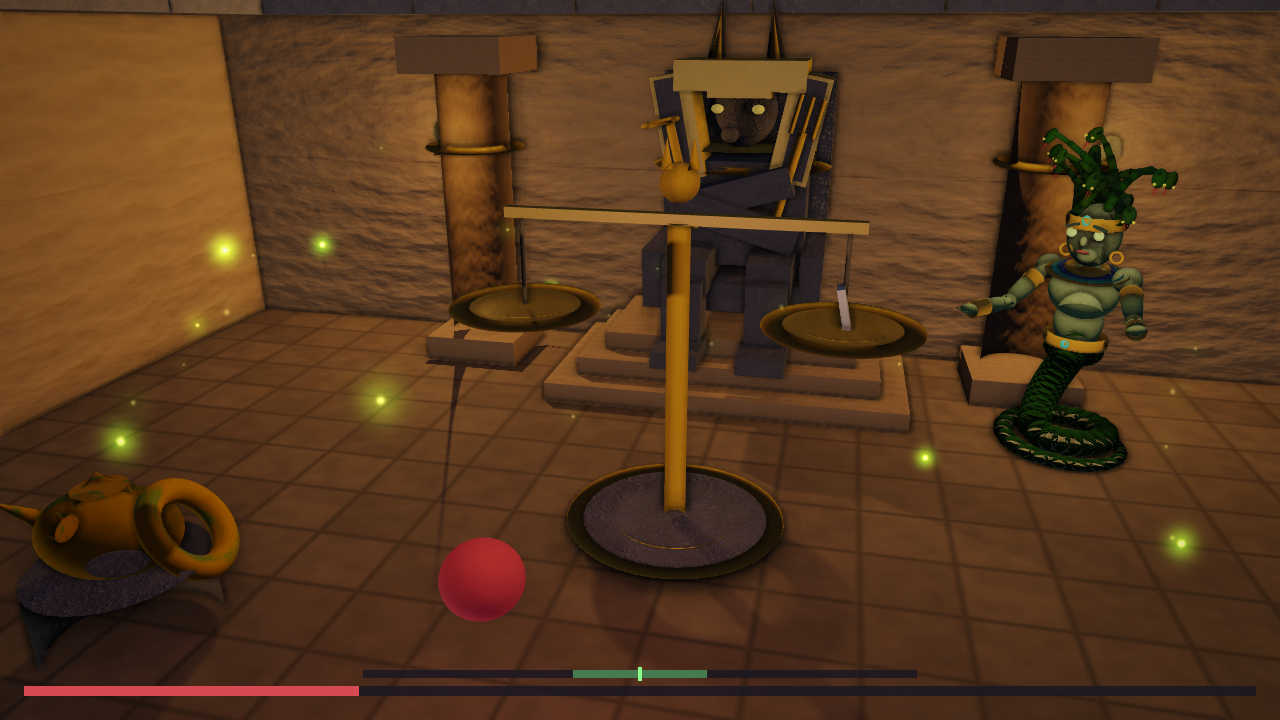
\includegraphics[width=0.82\textwidth]{initial_scene.png}
    \caption{Initial chamber environment showing the traveller, Anubis trial
    area, architectural elements, lighting, and major interactive objects.}
    \label{fig:initial_scene}
\end{figure}

% ---------------------------------------------------------
% Chamber and interaction results (2 x 2)
% ---------------------------------------------------------

\begin{figure}[H]
    \centering

    \begin{subfigure}[t]{0.48\textwidth}
        \centering
        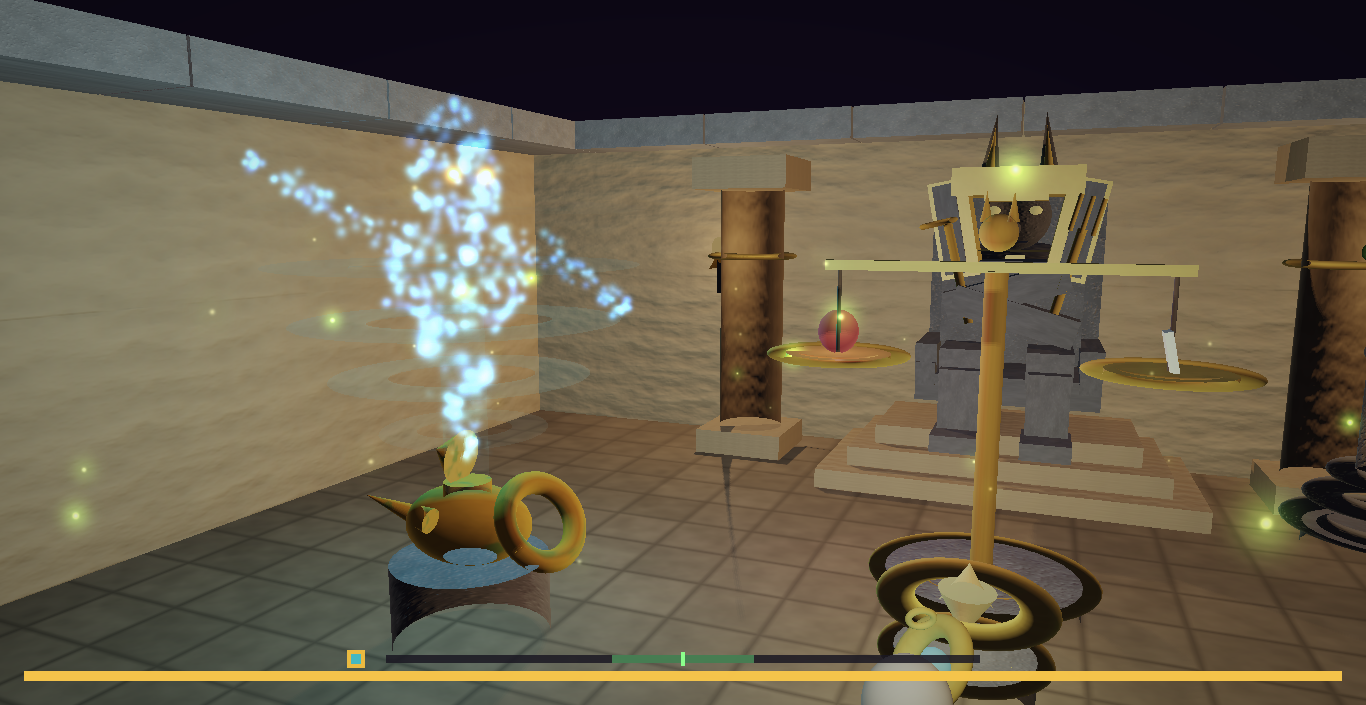
\includegraphics[width=\linewidth]{trial_djinn.png}
        \caption{Anubis trial and Djinn appearance.}
        \label{fig:trial_djinn}
    \end{subfigure}
    \hfill
    \begin{subfigure}[t]{0.48\textwidth}
        \centering
        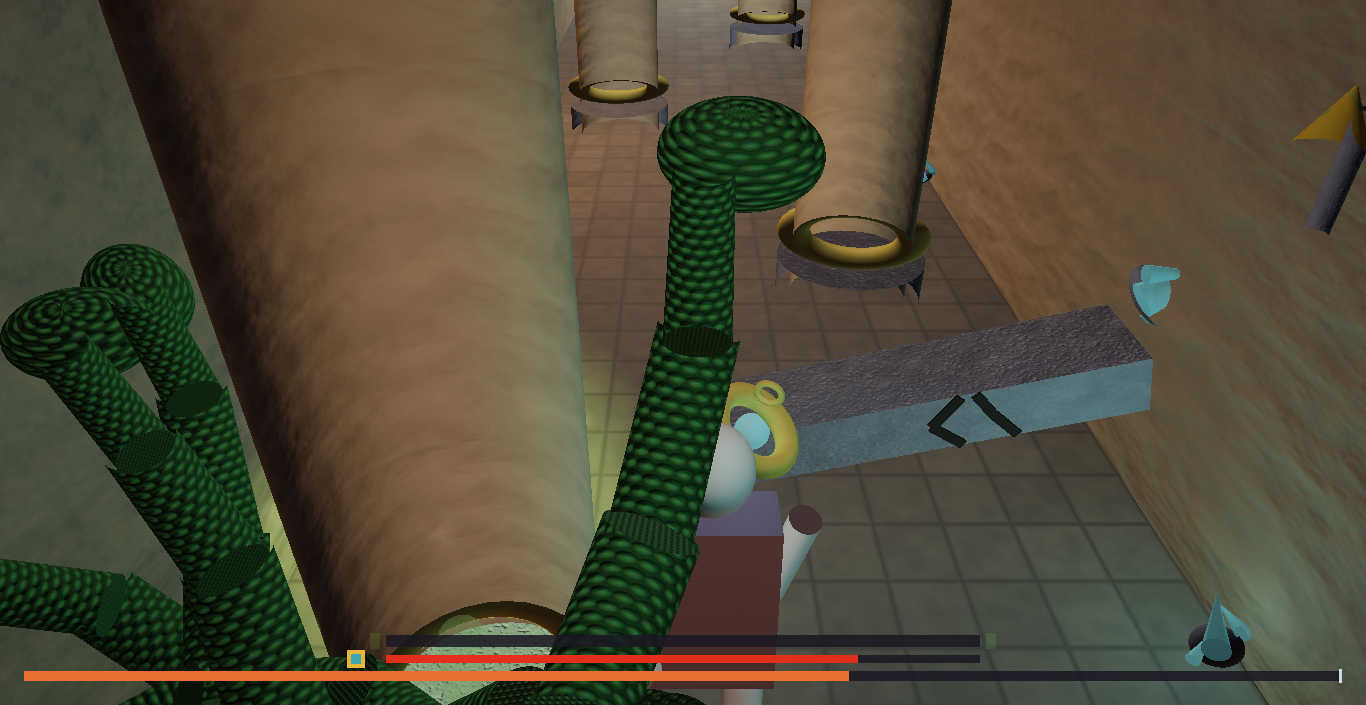
\includegraphics[width=\linewidth]{escape_medusa.png}
        \caption{Chamber collapse and Medusa pursuit.}
        \label{fig:escape_medusa}
    \end{subfigure}

    \vspace{0.25cm}

    \begin{subfigure}[t]{0.48\textwidth}
        \centering
        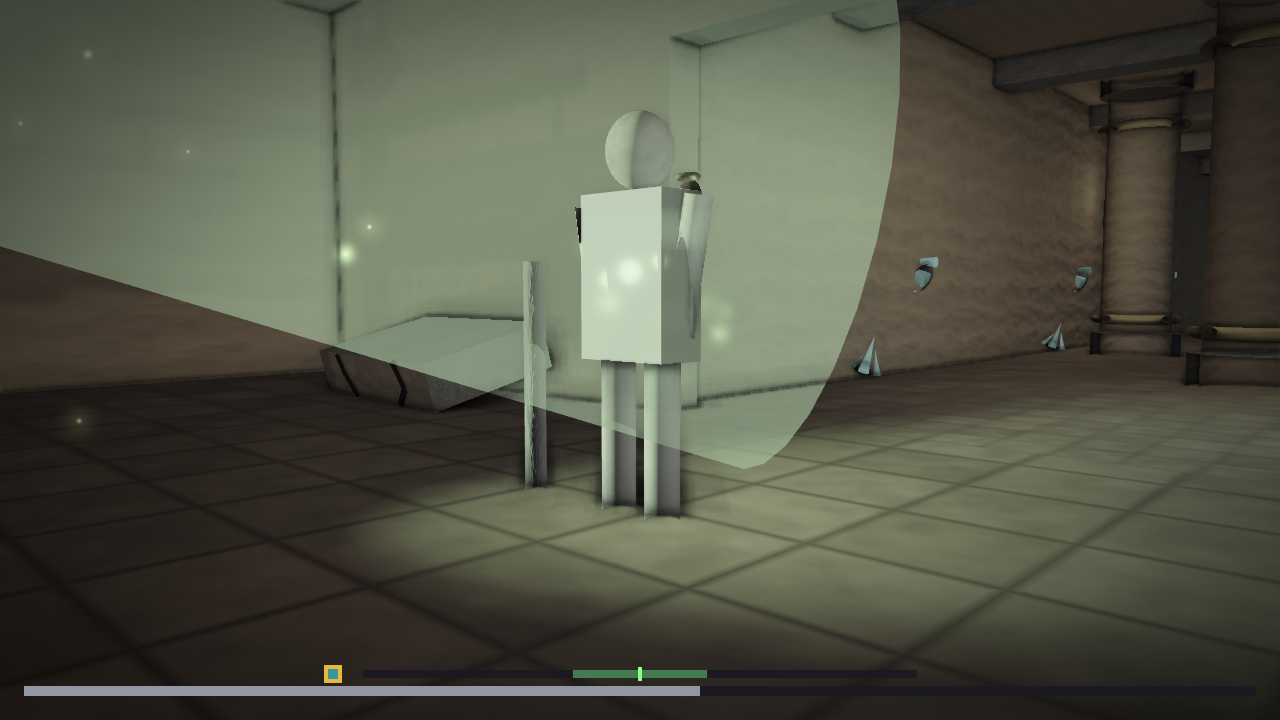
\includegraphics[width=\linewidth]{petrification.png}
        \caption{Progressive petrification caused by Medusa's gaze.}
        \label{fig:petrification}
    \end{subfigure}
    \hfill
    \begin{subfigure}[t]{0.48\textwidth}
        \centering
        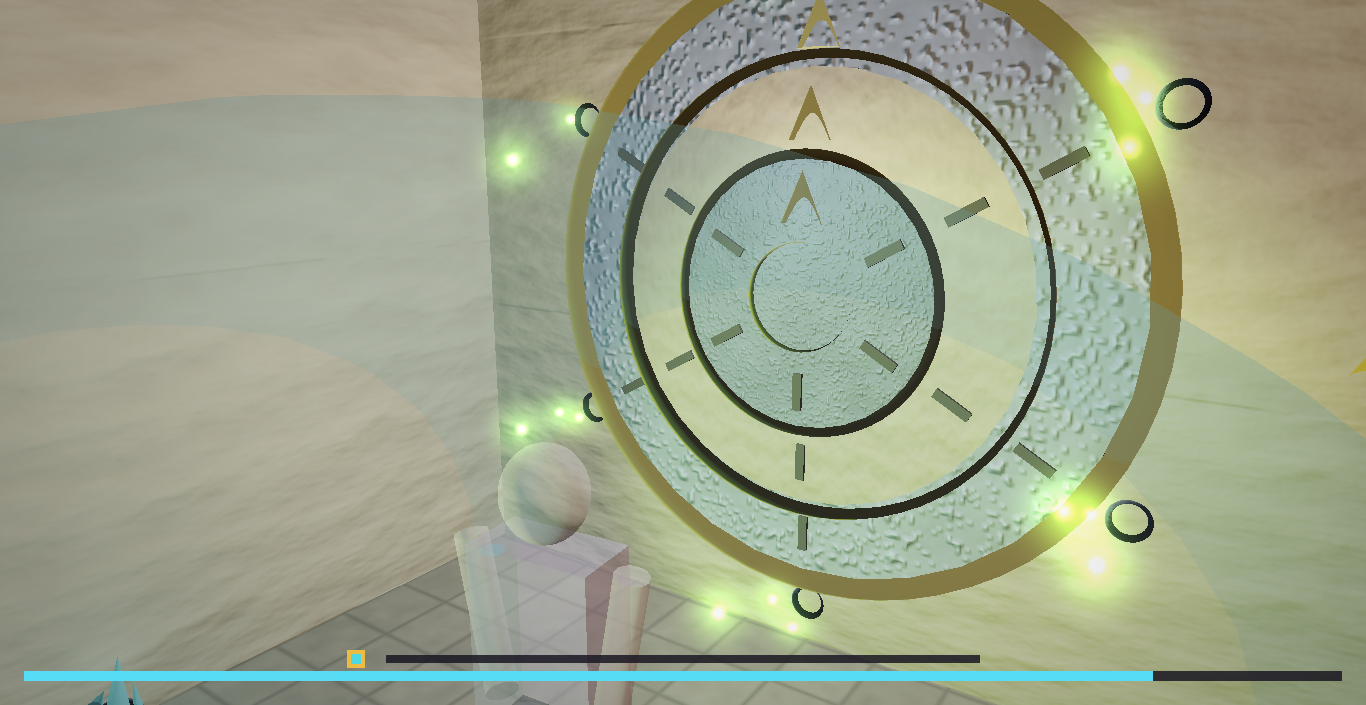
\includegraphics[width=\linewidth]{sanctuary_gate.png}
        \caption{Protective sanctuary and constellation gate puzzle.}
        \label{fig:sanctuary_gate}
    \end{subfigure}

    \caption{Major chamber-based interactions and visual effects:
    (a) hierarchical animation and particle-based Djinn formation,
    (b) environmental destruction and character pursuit,
    (c) flesh-to-stone petrification and curse effects, and
    (d) the protective sanctuary with the rotating-ring gate puzzle.}
    \label{fig:chamber_results}
\end{figure}

% ---------------------------------------------------------
% Garden and ascension results (2 x 2)
% ---------------------------------------------------------

\begin{figure}[H]
    \centering

    \begin{subfigure}[t]{0.48\textwidth}
        \centering
        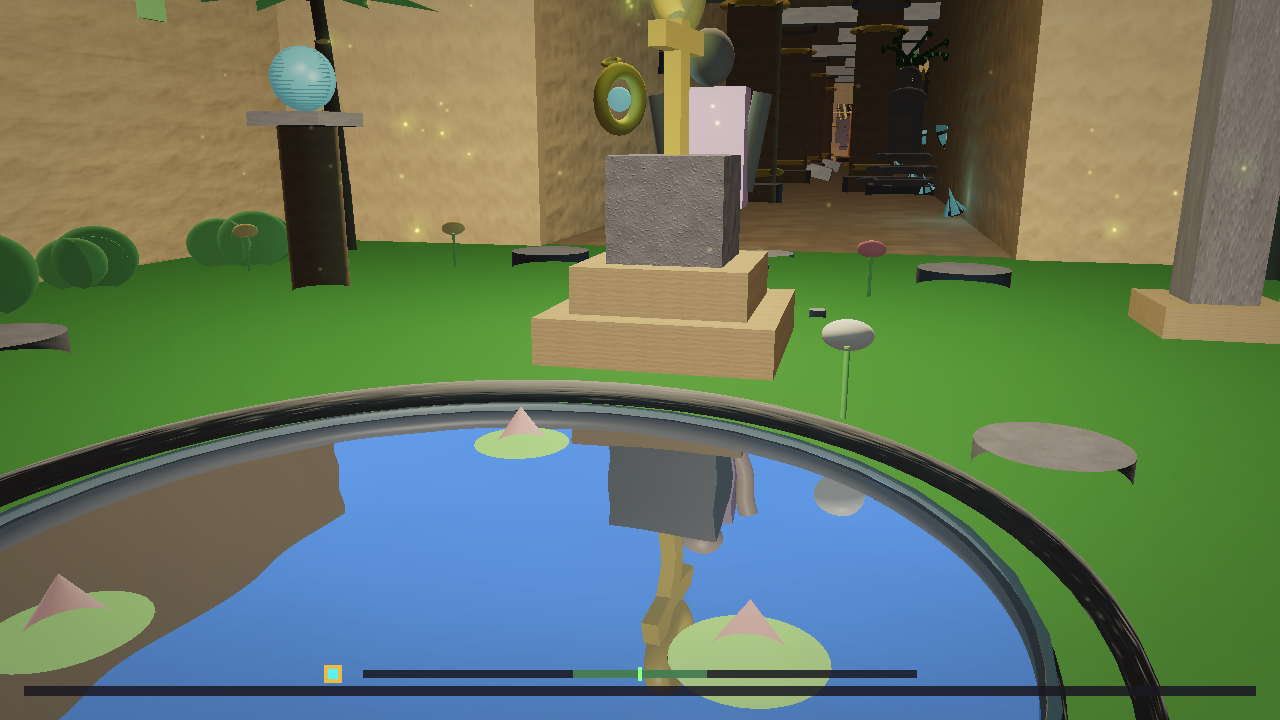
\includegraphics[width=\linewidth]{garden_dawn.png}
        \caption{Restored Garden of Lost Souls at dawn.}
        \label{fig:garden_dawn}
    \end{subfigure}
    \hfill
    \begin{subfigure}[t]{0.48\textwidth}
        \centering
        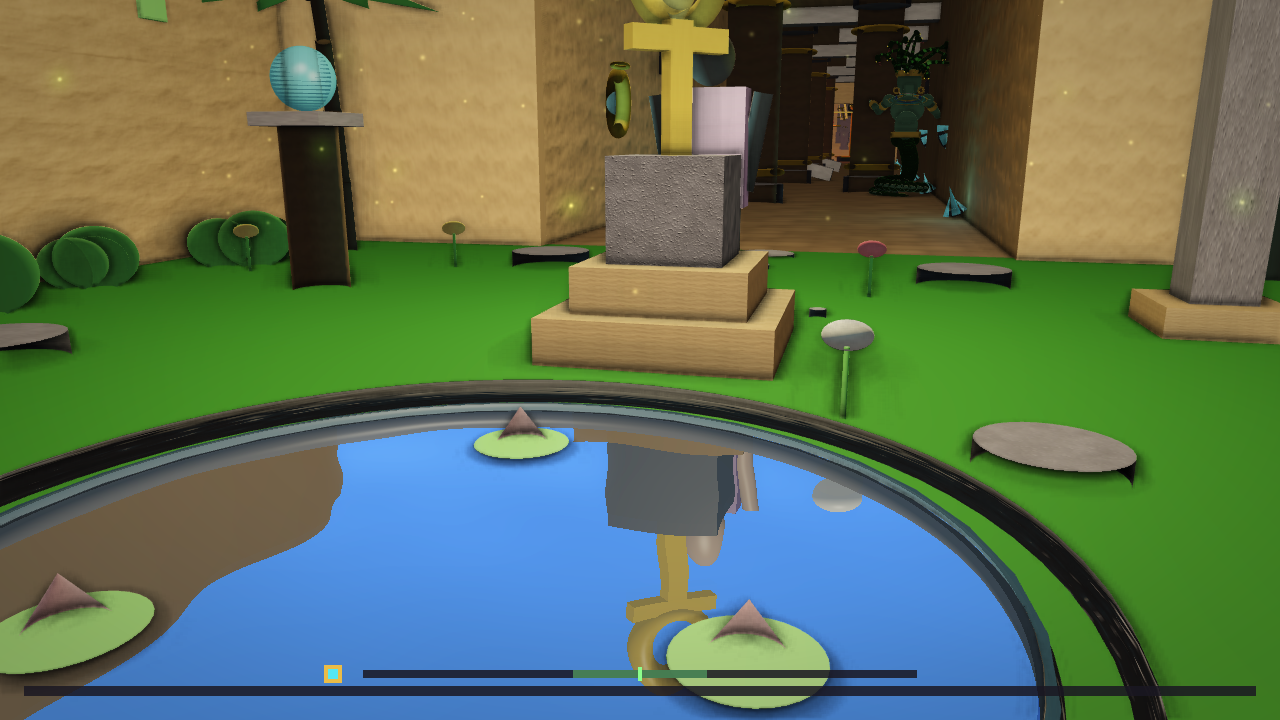
\includegraphics[width=\linewidth]{raytraced_pool.png}
        \caption{Ray-traced reflection on the garden pool.}
        \label{fig:raytraced_pool}
    \end{subfigure}

    \vspace{0.25cm}

    \begin{subfigure}[t]{0.48\textwidth}
        \centering
        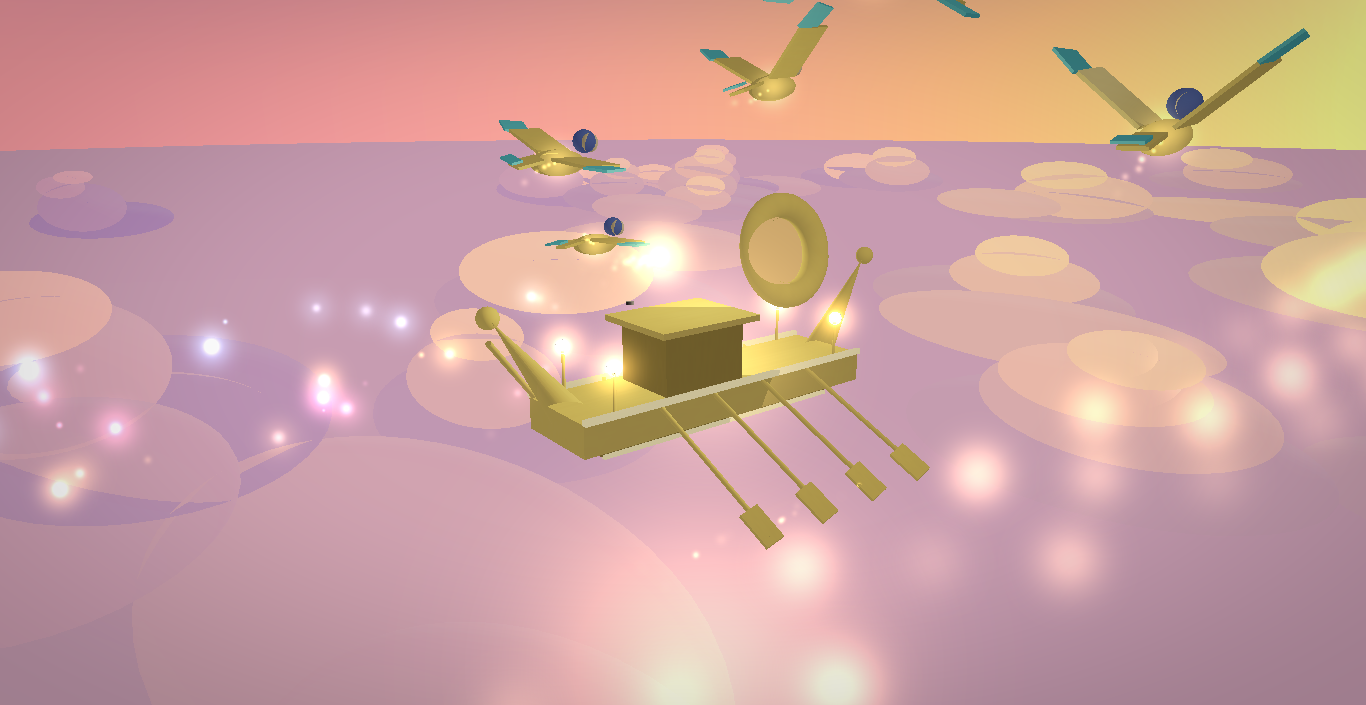
\includegraphics[width=\linewidth]{ascension_boat.png}
        \caption{River of souls and Ra's sun boat.}
        \label{fig:ascension_boat}
    \end{subfigure}
    \hfill
    \begin{subfigure}[t]{0.48\textwidth}
        \centering
        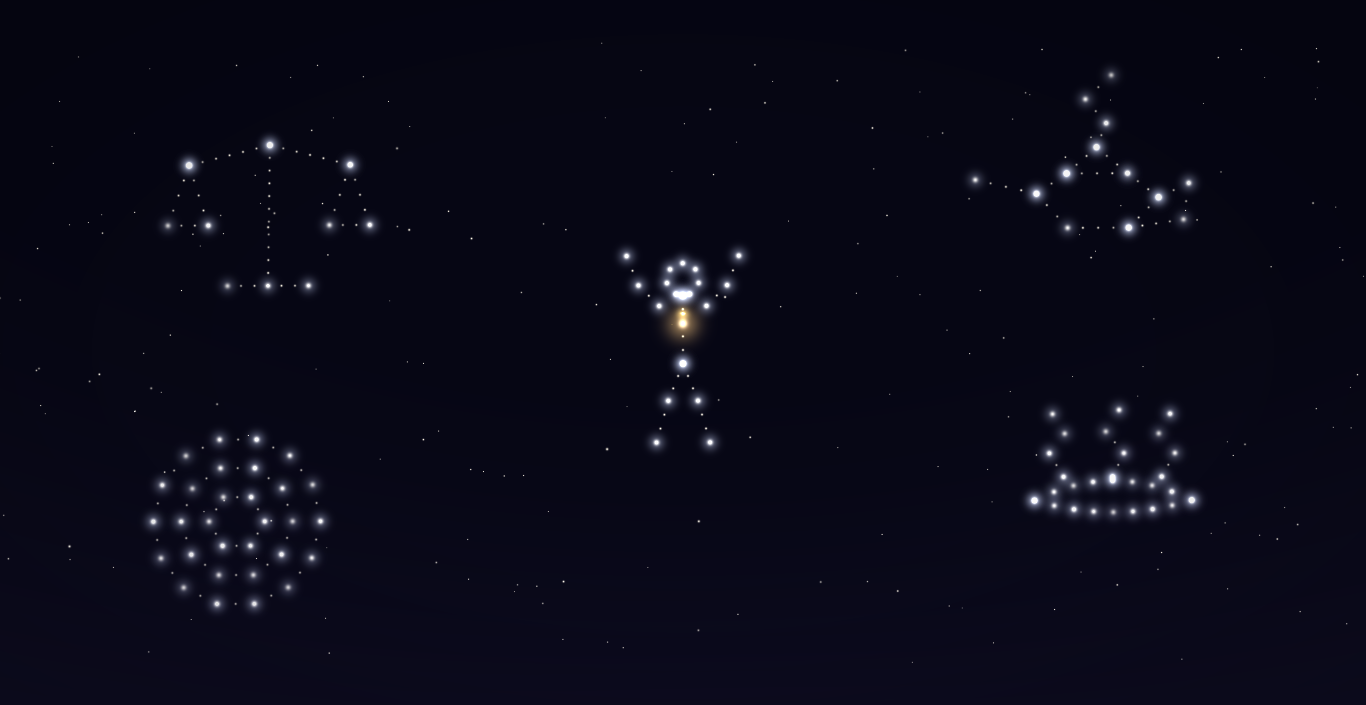
\includegraphics[width=\linewidth]{final_constellation.png}
        \caption{Final constellation and traveller's heart star.}
        \label{fig:final_constellation}
    \end{subfigure}

    \caption{Major garden and ascension results:
    (a) environmental restoration and dawn transition,
    (b) shader-based ray-traced water reflection,
    (c) the river of souls, Ra's sun boat and hierarchical animation, and
    (d) the final constellation sequence in which the traveller becomes a star.}
    \label{fig:garden_results}
\end{figure}

The screenshots show the visual development of the project from the original
chamber to the final celestial environment. The initial scene
(Figure~\ref{fig:initial_scene}) establishes the main 3D setting, while
Figure~\ref{fig:chamber_results} presents the principal interactive systems
inside the chamber. Figure~\ref{fig:garden_results} demonstrates the larger
environmental transformation after the gate, including garden restoration,
ray-traced reflection, soul animation, and the final ascension sequence.


% =========================================================
% 6. LIMITATIONS AND FUTURE WORK
% =========================================================

\section{Limitations and Future Work}

Although the project implements a large number of graphics and interaction
features, several systems intentionally use simplified methods so that the
complete application can run in real time and remain manageable within the
scope of the course project. Character and debris collision rely mainly on
simple geometric boundaries and circular obstacle regions rather than a full
rigid-body physics engine. Medusa uses direct pursuit with local obstacle
avoidance instead of a complete navigation mesh or global path-planning
algorithm, and large structural collapse follows designed animation stages
rather than physically simulated fracture.

The pool ray tracer also uses simplified scene geometry. Garden objects are
represented by boxes and ellipsoids rather than by their complete triangle
meshes. This makes reflection-ray calculations practical in the fragment shader
but reduces geometric accuracy for complex objects. A future version could use
triangle intersections together with an acceleration structure such as a
bounding-volume hierarchy. Larger particle systems could similarly be moved
from CPU-managed updates toward GPU-based simulation to support substantially
more particles during the Djinn, garden-soul, and ascension scenes.

Visual quality could also be extended with higher-detail external models,
additional physically based materials, improved animation blending, more
advanced water rendering, and stronger physical interaction between debris and
the environment. These improvements could be added without changing the core
design of the current application, which already separates scene objects,
gameplay systems, camera control, lighting, particles, and rendering.


% =========================================================
% 7. CONCLUSION
% =========================================================

\section{Conclusion}

\textit{The Trial of Three Curses} was developed as a complete interactive 3D
application in which computer graphics techniques directly support the
environment, interaction, and visual narrative. The project begins with the
contained Anubis trial but progressively expands into particle-based magical
effects, environmental destruction, character pursuit, a constellation puzzle,
a transforming garden, shader-based ray tracing, and a large cinematic
ascension. This progression made it possible to apply the same graphics
foundation to environments with very different visual requirements.

The implementation demonstrates geometric and hierarchical transformations,
model--world--view--projection processing, multiple camera modes, procedural
modeling, textured materials, tangent-space normal mapping, Blinn--Phong
lighting, directional, point, and spot lights, percentage-filtered shadow
mapping, particle animation, post-processing, per-fragment petrification,
collision and line-of-sight testing, dynamic environmental transformation, and
ray-traced reflection. These techniques are used throughout the Anubis scale,
Djinn, protective charm, collapsing chamber, Medusa encounter, sanctuary,
constellation gate, Garden of Lost Souls, wave of life, dawn transition, rising
souls, reflective pool, Ra's sun boat, Ba birds, and constellation finale.

The final project therefore demonstrates not only individual graphics
algorithms but also how those algorithms can be combined within a coherent
real-time application. The resulting environment connects graphics mathematics,
shader programming, animation, rendering, interaction, and visual storytelling
into a single continuous experience.


% =========================================================
% REFERENCES
% =========================================================

\begin{thebibliography}{9}

\bibitem{opengl}
Khronos Group,
\textit{OpenGL Reference Documentation}.

\bibitem{glfw}
GLFW Development Team,
\textit{GLFW Documentation}.

\bibitem{glad}
GLAD,
\textit{OpenGL Loader Generator and Documentation}.

\bibitem{glm}
G-Truc Creation,
\textit{OpenGL Mathematics (GLM) Documentation}.

\bibitem{learnopengl}
Joey de Vries,
\textit{LearnOpenGL: Learn Modern OpenGL Graphics Programming}.

\end{thebibliography}

\end{document}